\documentclass[12pt]{report}

\usepackage[utf8]{inputenc}
\usepackage{graphicx}
\usepackage{caption}
\usepackage{subcaption}
\usepackage{amsmath}
\usepackage{amsthm}
\usepackage{amsfonts}
\usepackage{float}
\usepackage[width=150mm,top=35mm,bottom=25mm,bindingoffset=6mm]{geometry}
\usepackage{fancyhdr}
\usepackage{algpseudocode}
\usepackage{commath}
\usepackage[normalem]{ulem}
\usepackage[toc,titletoc,title]{appendix}
\usepackage[nottoc]{tocbibind}
\usepackage{hyperref}

\useunder{\uline}{\ul}{}

\graphicspath{ {images/} }

\pagestyle{plain}
\fancyhf{}
\fancyhead[R]{\thepage}
\renewcommand{\headrulewidth}{0pt}
\setlength{\headheight}{15pt}

\title{Exploration and application of complex graph properties}
\author{Zi Yuan Chen}
\date{}

\begin{document}
\pagenumbering{roman} 

\begin{titlepage}
    \begin{center}
        \vspace*{1cm}
        
        \Huge
        \textbf{Exploration and application of complex graph properties}
        
        \vspace{0.5cm}
        \LARGE
        %Thesis Subtitle\\
        by\\
    
        \textbf{Zi Yuan Chen}
        
        \vfill

        \vspace{1.0cm}
        \begin{flushleft}
        \end{flushleft}
        
    \end{center}
    
\end{titlepage}

\chapter*{Abstract}
In this project, we study the background of graph theory and explain specific complex graph properties. These properties include trophic levels and coherence, the centrality values such as betweenness and closeness, the clustering coefficients and properties based on webpage traversal like HITs or page rank. Each are explored in detail with the methods of calculation based on various graph types. The graph type that we focus on is the directed graphs. This was chosen in consideration for linguistic analysis which I have undertaken in a later chapter. To analyse directed graphs based on the multiple formulas for each graph property, I have programmed a tool to generate graph visualisations. The tool uses the formulas for each graph property and calculates the relative value for each vertex in a graph. This can then be formalised into a dataset and used to generate graph visualisations. The vertex positions of the visualisations are amended based on the various graph properties. Positional changes is beneficial since it highlights key areas and certain correlations for the different languages that I have chosen to analyse. The languages in this project being English, German, French, Japanese, and Chinese. Detailed analysis of each language based on the graph properties is described in this project. Finally, the results are summarised with the future possibilities of graph analysis.

\chapter*{Acknowledgements}
Firstly, I would like to thank my supervisor Samuel Johnson for supporting me and introducing me to Graph Theory and the areas in which he has studied. For guiding me and giving his views throughout my explorations in Graph Theory. Taking the time to discuss and listen to what I've accomplished at various stages of this project and the next stages. As well as providing feedback on my findings and progress. I would also like to thank Sara Jabbari for her interest in my project and providing me with detailed feedback on what to improve.

Finally, I also thank my family and friends for supporting me and encouraging me through the project.



\tableofcontents

\listoffigures

\listoftables


\chapter{Introduction}
\pagenumbering{arabic} 
\section{Overview}
The application of mathematics has played a key role in the development of technological advancements and breakthroughs in science. Throughout history, mathematics has provided us with an increasing number of various sub-branches such as discrete mathematics, applied mathematics, cartesian geometry, algebra, calculus and many more. All of which can be applied to the real world, whether it is for construction, physics, or simple day-to-day activities. 

A key branch under discrete mathematics is graph theory where models can be developed to represent relationships between different objects. Graphs contain a range of uses both in the mathematical world and the real world. They can be used to visually represent large sets of numerical data providing a way to deduce different properties and the correlations they have within the data. Examples include identifying clustering of certain areas, the connectivity between vertices or edges and many others. Graphs are also widely known as networks with some examples such as a friendship network, business networks and even food chain levels. Graph theory is the area that I will explore along with a method to visualise them through the help of using python. As well as analysing specific properties that may influence the visualisation of the graphs and thus the outcome of any key relationships between the vertices.

\section{History}
Initially, graph theory was introduced in 1735 as a form of a solution to the seven bridges of Königsberg problem which was solved by Leonard Euler \cite{POWELL20151}. This famous problem involved an island within Königsberg that had a river, Pregel, surrounding the island via a fork. There were seven bridges that crossed the river Pregel from the island to connect to other major landmasses of Königsberg, Prussia. The island had four bridges, two north, two south connecting the mainland and the island. Also another bridge connecting to a neighbouring island and this neighbouring island itself had two bridges. Consequently, giving a total number of seven bridges as stated by the seven bridges of Königsberg problem, see Figure \ref{fig:Königsberg's Bridges}. 

Due to the location in which the island was situated, the problem was to determine whether a route exists that manoeuvres through all the bridges exactly once and must return to the starting location. Leonard Euler proceeded to analyse the problem by evaluating only the key areas, this was the land masses and the bridges. Other information such as the sizes of the island, bridge type or length were irrelevant. Consequently, the problem could be portrayed by utilising dots and lines to give a simplistic view (see Figure \ref{fig:Königsberg's Graph}). Once developed, the dots are known as vertices which represent the key interests and the edges that are incident to these vertices represents the connections/relationships between them.

By removing the irrelevant information, Euler was able to simplify and visualise the problem. In doing so, Euler discovered the fact that for a solution to exist, each vertex must have an even number of edges incident to them (even degree). This is because you require one edge for entering and another for exiting. Otherwise not all edges will be included in the final path that is based on the conditions of the bridge problem. All vertices in the Königsberg problem have odd degree, meaning that a \emph{Eulerian path} (a path that traverses all edges exactly once) does not exist for this problem. Since a Eulerian path does not exist then a \emph{Eulerian circuit} (a Eulerian path that returns to the starting vertex) cannot exist either. Therefore, Euler proved that there were no solutions to the seven bridges of Königsberg problem. This proof is regarded as the first proof in relation to graphs and led to the birth of graph theory.

\begin{figure}[!htb]
\centering
\begin{subfigure}{.45\textwidth}
	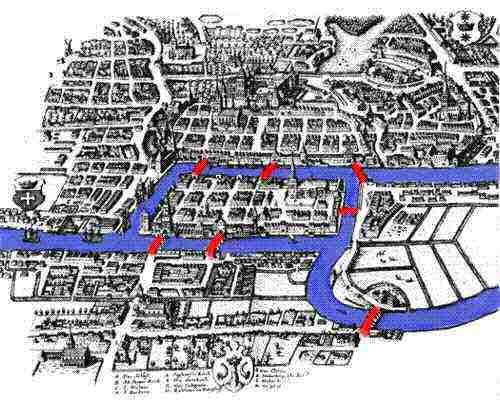
\includegraphics[scale=0.4]{Konigsberg}
	\caption{Königsberg and the seven bridges, from MacTutor Archive \cite{MacTutor}.}
	\label{fig:Königsberg's Bridges}
\end{subfigure}
\hfill
\begin{subfigure}{.45\textwidth}
	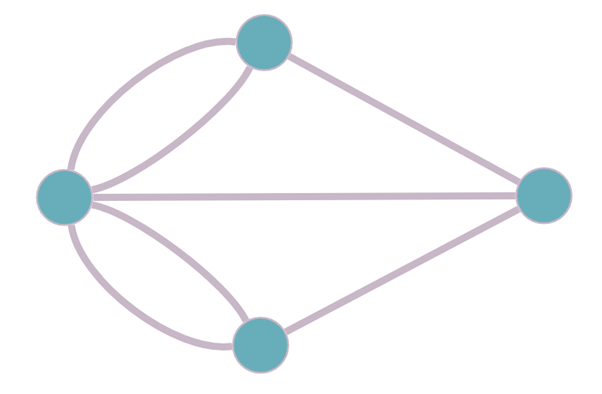
\includegraphics[scale=0.45]{Konigsgraph}
	\caption{Graph representation to Königsberg problem.}
	\label{fig:Königsberg's Graph}
\end{subfigure}
\caption{The original seven bridges of Königsberg and its graph representation that only focusses on the key details and disregards the irrelevant information. Achieved by using vertices and edges.}
\end{figure}

After Eulerian paths and cycles were introduced, the next famous puzzle in relation to graph theory was invented in 1857 and was known as the Icosian Game \cite{carlson_2022} by William Rowan Hamilton. The objective of the puzzle was to find a cycle that visits all vertices exactly once and returns to the starting vertex. This type of cycle is later defined as a \emph{Hamilton cycle} along with the definition of a \emph{Hamilton path} which does not have the requirement to return to the starting vertex.

In the mathematical world, Leonard Euler is known for \emph{Euler's identity} in complex mathematics which states that for a real number $x$, $e^{ix}=\cos(x)+i\sin(x)$. This has been crucial in many subject areas such as physics and engineering. Additionally in 1850, Euler uncovered another formula to be known as \emph{Euler's polyhedra formula} which states that $F + V - E = 2$ where $F$ denotes the number of faces, $V$ as the number of vertices and $E$ as the number of edges for a graph model. As polyhedrons can be depicted as graphs, algebraic topology benefited from Euler's polyhedron formula where more complex surfaces could be studied such as the surface of a torus. Based upon this formula, the \emph{Euler characteristic} was formalised to describe the topological characteristic of various complex surfaces with its formula as $F + V - E = 2 - 2g$ where $g$ is denotes the number of ``holes" the surface has (formally known as the \emph{genus}). 

Furthermore, graph theory has assisted in problems such as the four-colour map problem which was introduced in the 1850s. The problem asks if all the countries in the world can be coloured with only the use of four colours such that no two adjacent countries were coloured with the same colour. In which the solution was not found until 1972 by Kenneth Appel and Wolfgang Haken \cite{Ohnishi2009} through the assistance of a computer. An alternative example of a four colour problem is the colouring of the counties in the UK with only four colours where the solution for this is shown in Figure \ref{fig:UK 4 colour}.

\begin{figure}[H]
\centering
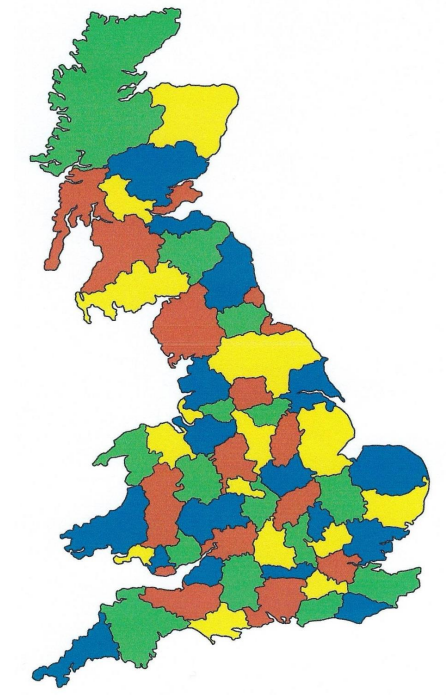
\includegraphics[scale=0.35]{4colourUK}
\caption{The solution for the four colour map problem with regards to the counties in the UK sourced from Robin Wilson \cite{4ColourRobin}.}
\label{fig:UK 4 colour}
\end{figure}

The Chinese postman problem is another such graph theory problem where you must find the shortest path that uses all the edges in the graph at least once. A similar alternative version is called the travelling salesman problem. In which you identify a shortest path that uses all edges exactly once in the graph and must end at the starting vertex. These such problems are used in Linear programming to find optimal solution in routing or pathing between locations. Variants of the CPP (Chinese postman problem) includes undirected Chinese postman problem (UCPP) and contains different restrictions depending on the subset of edges used (see the paper \cite{IrnichStefan2008Uppw}). Also there exists the Chinese postman problem with load-dependent costs (CPP-LC \cite{CorberánÁngel2018TCPP}) that includes weights on the edges so that an optimal route can be generated. This can widely be used and applied to problems such as the best route in order to lower a vehicle's CO$_2$ emission. These problems can be applied to modern day scenarios which means that they are still valuable to companies now.
\newline

Therefore, studies within graph theory have been researched extensively since 1735 with many beneficial factors brought into the real world. This is possible due to the versatile nature that data structures in the real world can be represented as mathematical structures through graphs or networks. Examples of what they can represent ranges from simple relationships between people to the complex structure of the brain by studying the brain's anatomic structure and assigning vertices according to the sections of the brains and edges as the links between them. The links are typically representations of the neurons in the brain. Further details of brain mapping into graphs can be read by the paper \cite{articlebrain}. Therefore, by using graph models, various patterns and correlations can then be derived to generate graph properties. These properties can be studied to develop useful information and possible improvements to the whole graph.

\section{Basic notation and terminology}
Graphs or networks are mathematical constructs that are formed by a collection of vertices and edges. Vertices $V$ represents individual objects such as land masses, companies, houses, people, etc. Edges $E$ represents the connections between the vertices such as their relationship, flow of water, supply chain, etc. Sets $V(G)$ or $V$ and $E(G)$ or $E$ forms the graph $G$ and can be written as $G=(V, E)$ with E being a subset of $V \times V$. So an edge $e \in E$ can be written as $v_{1}v_{2}$ if $e$ connects $v_{1}$ and $v_{2}$ where $v_{1}, v_{2} \in V$. There exist variations among graphs as they can be directed or undirected, the edges may carry weights and they may contain self-loops. Figures \ref{fig:Simple Graph} and \ref{fig:Directed Graph} show simple graphs, one of which is undirected, and another is directed. A graph $H = (V', E')$ is a \emph{subgraph} of $G=(V, E)$ if $V' \subset V$ and $E' \subset E$.

\emph{Order} is the mathematical term that represents the number of the vertices in the vertex set $V(G)$. \emph{Size} is number of edges or vertex pairs in the edge set $E(G)$. The \emph{degree} of a vertex, denoted by $deg(v)$ is the number of edges that are connected (otherwise known as \emph{incident}) to the vertex, discussed previously in Euler's solution to the seven bridges of Königsberg problem. Additionally, $\delta(G)$ and $\Delta(G)$ represents the \emph{minimum} and \emph{maximum degree} in $G$ respectively. $G$ is a \emph{regular} graph if $\delta(G) = \Delta(G)$. Vertices $v_{1}$ and $v_{2}$ are \emph{adjacent} if there exists an edge $e \in E$ that connects them. Vertex $v_{2}$ is also known as a \emph{neighbour} to $v_{1}$ and is part of the set $N(v_{1})$ which denotes the neighbours of $v_{1}$. 
\newline

\begin{figure}[!htb]
\centering
\begin{subfigure}{.45\textwidth}
	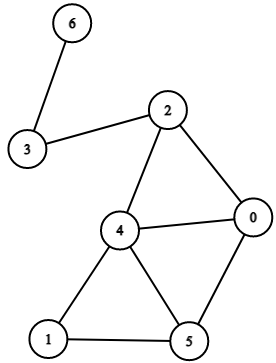
\includegraphics[scale=0.8]{simplegraph}
	\caption{An undirected graph with 7 vertices, 9 edges and an average vertex degree of $18/7$.}
	\label{fig:Simple Graph}
\end{subfigure}
\hfill
\begin{subfigure}{.45\textwidth}
	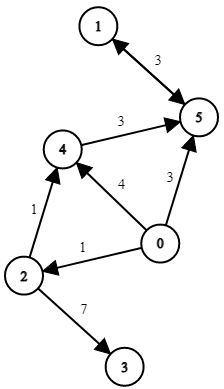
\includegraphics[scale=0.8]{directedgraph}
	\caption{A directed graph with 7 vertices and 7 directed edges that contain weighted edges.}
	\label{fig:Directed Graph}
\end{subfigure}
\caption{The two simple types of graphs within graph theory that are the basic building blocks for more complex structures and theorems.}
\end{figure}

There are multiple ways to traverse a graph. A \emph{walk} $w = v_1v_2v_3v_4v_5...v_n$ is a sequence of vertices such that $E(w) = (v_1v_2,...,v_{n-1}v_n)$ where vertices and edges can be revisited. They can be \emph{open} or \emph{closed} depending on whether the final vertex is equal to the starting vertex, open if equal and closed if not. A \emph{trail} is an open walk where no edges are revisited but vertices may be revisited. When all the edges are traversed exactly once, it is known as a \emph{Eulerian trail} (mentioned previously as a Eulerian path) and the graph is called \emph{semi-eulerian} or \emph{traversable}. Similarly for a trail that is closed (returns to the start), then it is known as a \emph{circuit} and if all edges are used then it is called a \emph{Eulerian circuit} (or Eulerian cycle) and the graph is defined to be \emph{Eulerian}. A \emph{path} is a trail but with no vertex repetitions and if the size of the path is equal to the size of the graph, then it is a \emph{Hamilton path}. Finally, a \emph{cycle} is a path that ends at the starting vertex and if all vertices are visited exactly once, then it is known as a \emph{Hamilton cycle} meaning that the graph is \emph{Hamiltonian}.
\newline

When considering network with flows, vertices can be known as nodes and may have capacities that limit the overall flow through the network shown in Figure \ref{fig:Network Flow}. These networks are especially used when considering plumbing, water pipes and even evacuation routes in a building. Within a room there is a capacity that is represented by the node's capacity and the weights of the edges can demonstrate the rate of flow along with its maximal flow. In other words, when people are evacuating a building, the corridors have a limit to the amount of people that may pass through. Networks can be used to model social network processes through the study of small corporate groups to generate a communications network. This network representation will have a flow of sentiments based on social network theory \cite{ZACHARY1984259} that is constrained in three ways. Firstly, by any existing direct relationships within the group, that will be denoted by vertices. Secondly, the frequency of communication of the relationships defined in the first point. Lastly, the breadth of the existing relationships in the network. Thus, by using graphs and networks, social behaviours within groups or companies can be studied giving ways to more phycological information represented by numerical data.

\begin{figure}[!htb]
\centering
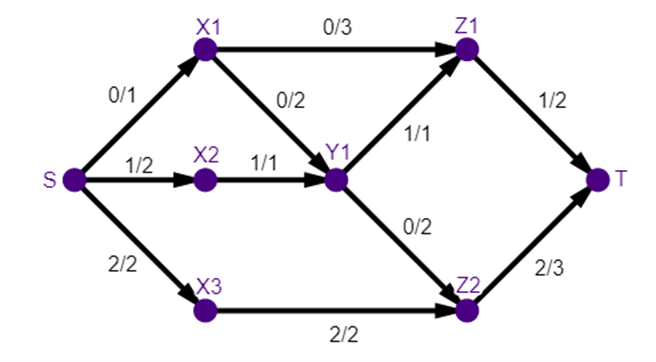
\includegraphics[scale=0.8]{networkflow}
\caption{A simple network flow with a source node and a sink node, the current flow is 3 and the edge capacities are shown.}
\label{fig:Network Flow}
\end{figure}

Additionally, graphs can be represented by the use of matrices to enable the use of matrix calculations on the datasets. These matrices are known as \emph{adjacency matrices} \cite{KnauerU.2011Agt:} and this matrix contains the number of edges incident to each vertex. The connections of the vertices are based on the location of this value as the rows and columns represent the vertices. A \emph{weighted adjacency matrix} will instead hold the weights of each edge in the matrix. An $n \times n$ adjacency matrix $A = (a_{ij})$ for $ i, j = 1, ..., n$ is defined by $a_{ij} = 1$ if there exists an edge from vertex $i$ to vertex $j$. A matrix is always symmetric when considering an undirected simple graph as an edge will contribute to both sides of the matrix. Examples of an adjacency matrix along with its graph representation is shown in Figure \ref{fig:Adjacency Graph}.
\newline

\begin{figure}[!htb]
\centering
$\vcenter{\hbox{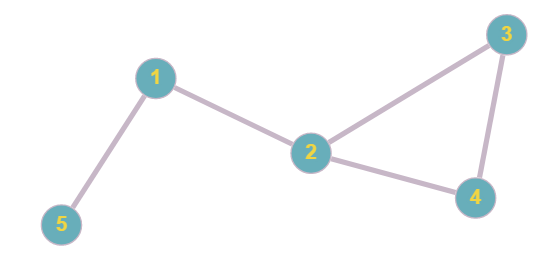
\includegraphics[scale=0.6]{adjgraph}}}$
\hfill
$A = \begin{pmatrix}
0 & 1 & 0 & 0 & 1 \\
1 & 0 & 1 & 1 & 0 \\
0 & 1 & 0 & 1 & 0 \\
0 & 1 & 1 & 0 & 0 \\
1 & 0 & 0 & 0 & 0 \\
\end{pmatrix} $
\caption{A simple graph along with its adjacency matrix.}
\label{fig:Adjacency Graph}
\end{figure}

The focus for future chapters will be on directed graphs and the data that can be extracted from them. Chapter 2 will describe and outline specific complex graph properties that will be applied to datasets later. This means that by analysing the graphs, numerical values can be generated to represent certain factors of the graph. These factors can then be applied to the graph to rearrange its shape so that further correlation can be identified between all the vertices and edges. Ideally, we will explore lexical analysis and study datasets generated based on different languages. But to achieve this, we will first discuss the graph properties that could assist in identifying correlations before the language datasets.

\chapter{Graph Properties}
There exist many different graph properties that can be applied depending on the specific graph type. Hence, we will focus on properties that can be applied to connected graphs to provide a collection of values targeted for the same layout structure and giving a wider selection of these such properties. Our aim is to apply these properties onto lexical graphs to enable the analysis of languages. To accomplish this, each property must be able to calculate their values in a connected graph that can be directed. So, a detailed study of each property will be given and the graphs that they can be applied to. 

\section{Trophic Coherence}
We begin with the graph property of \emph{trophic coherence} \cite{johnson2014trophic}, this property determines the stability of the graph and provides \emph{trophic levels} to individual vertices within the graph. Trophic levels are taken from ecology and applied to graphs to generate a height-based format for the vertices of a graph. Thus, for a connected directed graph $G =(V,E)$, we have $V$ which is the set of all vertices in $G$ and $E$ which is the set of all the edges within $G$. The graph can be represented with an adjacency matrix $A$ where $a_{ij}$ denotes the elements within the matrix. The standard trophic level definition on vertices uses the in degree and the out degree of the vertex $v_i$ given by Equation \ref{eq:inoutt}.

\begin{equation} \label{eq:inoutt}
k_i^{\text{in}} = \sum_ja_{ij} , \qquad \qquad k_i^{\text{out}} = \sum_ja_{ji} 
\end{equation}

The standard trophic level formula for vertices $v_i \in V$ is defined as:

\begin{equation}
t_i = 1 + \frac{1}{k_i^{\text{in}}}\sum_ja_{ij}t_j
\end{equation}

By ecological convention, $t_i = 1$ if the vertex $v_i$ is \emph{basal}. A vertex is known to be basal if it has no edges directed to it, i.e., $k_i^{\text{in}} = 0$. The trophic level equation can also simply be written in matrix form by Equation \ref{eq:mtl} with $\bold{z}$ defined as $z_i = \text{max}(k_i^{\text{in}},1)$ and $\Delta = \text{diag}(\bold{z}) - A$.

\begin{equation} \label{eq:mtl}
\Delta\bold{t} = \bold{z} 
\end{equation}

All vertices will receive a trophic level if and only if the Laplacian matrix $\Delta$ is invertible as the row sum of elements in $\Delta$ equals 0 for non basal vertices. If there are no basal vertices in the graph then $\Delta$ will be equal to the zero matrix and thus be singular, i.e., no inverse. This is discussed by Samuel Johnson \cite{johnson2020digraphs} in the investigation of stability and such dynamical features within graphs. So, for standard trophic levels equation to be applicable for the entire graph, there must exist at least one basal vertex meaning that this is a limitation to the definition of trophic levels. In the case of lexical analysis, a basal vertex exists because sentences will always have a word that is the start, i.e., a vertex without any in edges. However, in a larger dataset, the starts of sentences may be used in other areas meaning that they are no longer basal. Consequently, we study the improved equation for trophic levels and the possibility of weight inclusion. 

\subsection{Inclusion of weights and equation improvement}
In a weighted graph $G = (V, E)$, edges carry a weight between a vertex $v_i$ to a vertex $v_j$ where $i , j = 1 , 2, \dots , \lvert V \rvert$. Weighted matrix $W$ are used as a representation of the entire graph along with incorporating the direction of each edge and self-loops if they exist. The elements of the weighted matrix are $w_{ij}$. If the graph is not weighted then the edge is valued as 1 if the edge exists and 0 otherwise, i.e., the adjacency matrix of G. The total weight (also known as the \emph{strength}) for each vertex is defined by the weights into a vertex $v_i$ and the weights out of vertex $v_i$, which is shown by $s_{v_i}$ in Equation \ref{eq:strength}. This is essentially the same as the in and out degrees of Equation \ref{eq:inoutt} mentioned previously but instead of 1s and 0s, the weighted values are considered. The imbalance of the vertex $v_i$ is defined by the weights in of a vertex minus the weights out of the vertex shown by $i_{v_i}$ in Equation \ref{eq:imb}.

\begin{align}
s_{v_i} &= \sum(w_{v_iv_j}) + \sum(w_{v_jv_i}) \label{eq:strength} \\
i_{v_i} &= \sum(w_{v_iv_j}) - \sum(w_{v_jv_i}) \label{eq:imb}
\end{align}

Vectors $\bold{s}$ and $\bold{i}$ hold all the values of the strength and imbalance for all vertices respectively. We let $\bold{h}$ be a vector, then the graph Laplacian operator in matrix form is defined by Equation \ref{eq:delt}.  

\begin{equation} \label{eq:delt}
\Delta = \text{diag}(u) - W - W^T
\end{equation}

Therefore to get the trophic levels for each vertex with consideration for the additional weights, we solve the system of equations for vector $\bold{h}$ as shown by Equation \ref{eq:h}.

\begin{equation} \label{eq:h}
\Delta \bold{h} = \bold{v} 
\end{equation}

The values within this vector $h$ correspond to the trophic levels for the relative vertices. The values are used to illustrate the various trophic levels within a graph to give a hierarchical format visualisation. Trophic levels are not unique solutions because an arbitrary constant can be added to each component of the graph if there are multiple components to generate new levels that would be correct. The benefit to this is that Equation \ref{eq:h} can use an arbitrary constant $c$ for a vertex in $\bold{h}$ to influence the value of other vertices in a component. If there are multiple components to the graph, then a vertex in each component is needed. A unique solution can be found this way in which the trophic level values can be shifted so that a better graphical display can be generated. For example, having the lowest trophic level to be 0. 

Trophic levels can also be used to equate the overall \emph{trophic incoherence} of the graph rather than just looking at the graph on a vertex level. By using the trophic levels from $\bold{h}$, the equation for the trophic incoherence is defined by R. S. MacKay, S. Johnson, B. Sansom \cite{johnson2020digraphs} to be:

\begin{equation}
F_0=\frac{\sum_{v_iv_j}w_{v_iv_j}(h_{v_j}-h_{v_i}-1)^2}{\sum_{v_iv_j}w_{v_iv_j}}
\end{equation}

The possible shifting of the trophic levels does not affect the trophic incoherence meaning that the equation is independent. The incoherence is strictly ranged from 0 to 1. If $F_0 = 0$  then the graph is \emph{maximally coherent} as it would mean that all levels in the graph have a precise equal spacing which means that the graph is perfectly separated into levels. Whereas if $F_0 = 1$ then the graph is \emph{maximally incoherent} and levels are harder to decipher. As $F_0$ measure the incoherence, by taking $1 - F_0$, this would instead measure the coherence of the graph as they are each other's converses. 
\newline

In conclusion, trophic levels can be applied to weighted directed graph and any subcategories to achieve a hierarchical view of the graph. This eases the visualisation of many datasets and is used to decipher valuable information that may be of use. Through the combination of other graph properties which are described in this chapter, various combinations of these properties will yield different visualisations. This will prove beneficial in finding key vertices and correlations when analysing various languages. Through using trophic levels in languages, the graph can be formatted to demonstrate the sentence structure visually. Additionally, as shifting their trophic values does not affect the overall coherence, values can be modified so 0 indicates the start of the sentence and larger values indicate positions further up the sentence.

\section{Clustering Coefficient}
The \emph{clustering} of a graph, also known as \emph{transitivity} \cite{schank2005approximating}, is a property of a graph that measured the density of triangles within the graph. Triangles are where 3 vertices are connected. Clustering is used to quantify the graph's connectivity strength as it determines the fraction of triangles over the possible triangles that could be formed within the graph. Another perspective is that the coefficient quantifies the probability of a vertex $a$ having an edge to vertex $c$ if $ab$, $bc \in E(G)$. Thus, the \emph{clustering coefficient} determines how complete the graph is with a value of 1 meaning it is complete and 0 if not. There are two popular introductions of clustering coefficient, the \emph{local clustering}, and the \emph{global clustering}. The global clustering coefficient essentially measures the completeness of the graph by measuring the number of existing triangles divided by the number of possible triangles. The local clustering coefficient measures the clustering coefficient for each vertex rather than the whole graph. The measurement is taken by the number of triangles that has a connection to this vertex over the number of triples centred on this vertex. In other words, the local value demonstrates how close the neighbours of this vertex are to being a complete graph (a \emph{clique}).

\subsection{Clustering for simple graphs}
For simple connected graphs that are unweighted and undirected, we determine the coefficients of the clustering. The global clustering coefficient is defined by equation \ref{eq:sgcc} where $\sum{T}$ denotes the number of triangles (closed triplets) and $\sum{\tau}$ denotes the number of connected triplets in the graph.
\begin{equation} \label{eq:sgcc}
C = \frac{3\text{(Number of all triangles)}}{\text{Number of all connected triples}} = \frac{\sum{T}}{\sum{\tau}}
\end{equation}
An alternative equation which was demonstrated by M.E.J. Newman \cite{Newman_2003} through the studies of complex networks in terms of social networks. This is where the clustering coefficient determines the likelihood that a friend of your friend is also your friend. So, the alternative equation is written in the form of equation \ref{eq:sgccp} where $\sum{P_2}$ denotes the number of paths with length two within the graph.
\begin{equation} \label{eq:sgccp}
C = \frac{6\text{(Number of total triangles)}}{\text{Number of paths with length 2}} = \frac{\sum{T}}{\sum{P_2}}
\end{equation}

By considering the vertices of the graph, the local clustering coefficient can be defined to give such a coefficient to each vertex $v\in V(G)$ and is achieved by the equation \ref{eq:slcc} where $i$ is the index of the vertex. This definition is from paper \cite{Newman_2003} and proposed by Watts and Strogats \cite{Watts1998} where they analysed small world networks in relation to various real-world systems by the use of clustering coefficients and random graphs to formulate certain similarities. Note that if the degree of a vertex is 1 then the coefficient can be determined as 0, otherwise the equation will lead to $0/0$.
\begin{equation} \label{eq:slcc}
C_i = \frac{\text{Number of triangles connected to vertex $i$}}{\text{Number of triples centred on vertex $i$}}
\end{equation}

Another representation of the global clustering coefficient is to take the averages of all the local coefficients \cite{https://doi.org/10.48550/arxiv.1410.1997}. When the vertices have a degree of 0 or 1 then $C_i = 0$ so global clustering coefficient can also be defined by equation \ref{eq:sglcc}.
\begin{equation} \label{eq:sglcc}
C = \frac{1}{n}\sum_i{C_i}
\end{equation}
Later the clustering coefficients will be used as assistance to model graphs generated from a language dataset. However, to provide more accurate coefficients, variations of the clustering formulas will be defined based on the inclusion of weights and/or directions. In terms of our goal of lexical analysis, directions are of key importance since the word graphs will be directed. Therefore, the definitions of clustering coefficients must be developed further, starting with a overview of the inclusion of weighted edges.

\subsection{Clustering for weighted graphs}
Now by considering graphs as before but weighted instead, the equations undergo changes. For the instance of weighted graphs, there are multiple different definitions of clustering coefficients, each with slight variation in coefficients. This section will summarise a couple of the different definitions for weighted graphs and further detail can be analysed from Tanguy and Anna Levina on weighted directed clustering \cite{PhysRevResearch.3.043124}. In this paper, four different definitions are reviewed which are the Barrat definition, Onnela's definition, Zhang \& Horvath and their own continuous definition for weighted graphs. Zhang \& Horvath \cite{ZhangHorvath+2005} have used their definition of weighted clustering coefficients to analyse gene co-expression networks to review their functionality. Additionally, by soft or hard thresholding, it enables them to determine relationships between the clustering coefficient and gene networks within biology.

Alternatively, a simple idea to associate the clustering coefficient with regards to the edge weights is to define a value $w$ that represents the value of the triplet. $w$ can be the summation of the triplet, the mean of the triplet or another suitable method depending on the purpose. We take $w$ to be the summation of edges of the triplets. Then Equation \ref{eq:wcc} calculates the weighted clustering coefficient \cite{opsahl2009clustering} where $T$ denotes the triangles in the graph and $\tau$, the triples.
\begin{equation} \label{eq:wcc}
C = \frac{\text{Total of closed }w}{\text{Total of }w} = \frac{\sum_T{w}}{\sum_\tau{w}}
\end{equation}

\subsection{Clustering for directed graphs}

We see that weights can be added trivially through Equation \ref{eq:wcc}. So now considering the addition of directions as well as the possibility of weighted edges. Directions cause further complexities in the coefficients of clustering due to the various number of different \emph{motifs}. Motifs are various patterns in graphs that are reoccurring and can be used here to describe the nature of the triangles. For instance, there are 16 possible motifs for directed graphs of 3 vertices shown in Figure \ref{fig:3nodes}. However, if we consider only connected triangles, they can be organised into 4 types of motif groups known as \emph{Cycles}, \emph{Middleman}, \emph{Fan-in} and \emph{Fan-out}. Demonstrated by Figure \ref{fig:change} which are used in the study of higher order motifs and synaptic integration by Bojanek, Zhu and Maclean \cite{synaptic}. An interesting result used in this paper is the isomorphisms between the middleman, fan-in, and fan-out motifs.

\begin{figure}[!htb]
	\centering
	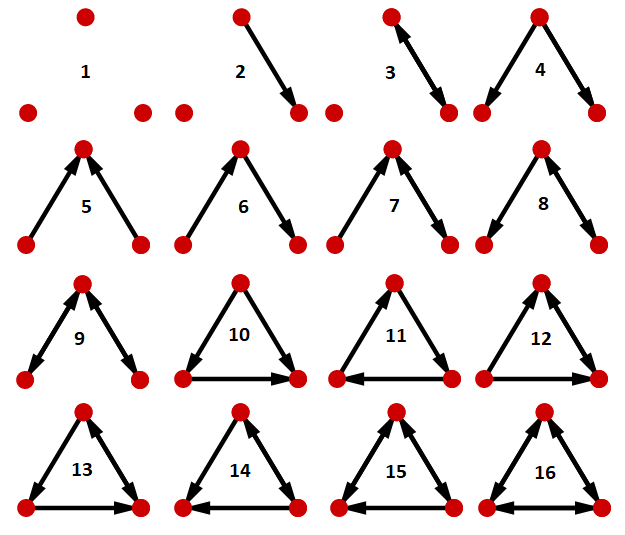
\includegraphics[scale=0.6]{3nodes}
	\caption{All 16 motifs of possible connections between 3 nodes and their directions shown on the edges. Ranges from 0 directed edges to the maximum of 6 directed edges.}
	\label{fig:3nodes}
\end{figure}

\begin{figure}[!htb]
	\centering
	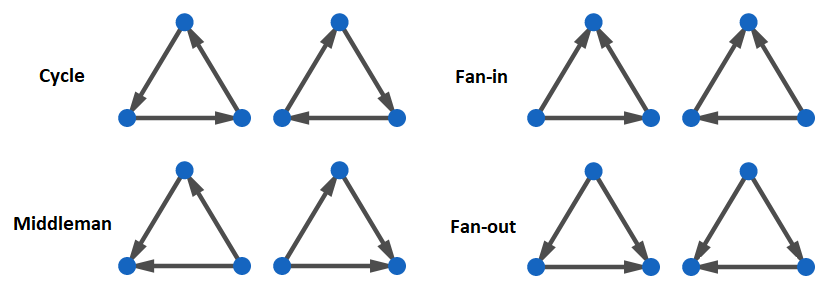
\includegraphics[scale=0.6]{change}
	\caption{The 4 named categories of motifs in which all directed connected triangles fall under. Each pair of motifs is listed as the corresponding types which are cycles, middleman, fan-in, and fan-out.}
	\label{fig:change}
\end{figure}

Consideration of the directional edges yields better accuracy in the coefficient values. One of the versions mentioned in the paper \cite{PhysRevResearch.3.043124} was Fagio's where he introduces the clustering coefficient to binary directed networks which are equivalent to simple directed connected graphs. Firstly, the equation for the directed version without the consideration of weights is defined by the ratio of all directed triangles centred on a vertex $i \in V(G)$ over the number of all possible triangles that could be formed with vertex $i$. Which are called $t_{i}$ and $T_{i}$ respectively. Before the directed equation for clustering, prior properties of the graph are necessary so that the equation can be easily formulated. Thus, consider a graph $G = (V, E)$ with its matrix representation as the adjacency matrix $A$ along with $V_1$ as the column vector, dimension $n$ of the graph, of only 1s. $A_i$ is the $i$-th row of the adjacency matrix. The in-degrees and out-degrees of a graph are the total number of edges going in or out of a vertex $i\in V(G)$ respectively, the total degree is the sum of the in and out degrees shown by Equations $\ref{eq:idod}$.

\begin{align} \label{eq:idod}
\text{in}(d_i) &= \sum_{i\neq j}a_{ji} = (A^T)_i V_1 \\
\text{out}(d_i) &= \sum_{i\neq j}a_{ij} = (A^T)_i V_1 \nonumber \\
\text{tot}(d_i) &= \text{in}(d_i) + \text{out}(d_i) \sum_{i\neq j}a_{ji} + \sum_{i\neq j}a_{ij} = (A^T + A)_i V_1 \nonumber
\end{align}

When the edge is directed both ways, this degree is the summation of the products of all the edges of vertex $v$ that are bidirectional. Formally can be shown as equation \ref{eq:bd} with $A_{ii}$ as the $i$-th element of the diagonal for the matrix product of $A$.

\begin{equation} \label{eq:bd}
\text{bi}(d_i) = \sum_{i\neq j}a_{ij}a_{ji} = A_{ii}^2 
\end{equation}
 
Equation \ref{eq:dcc} is demonstrated by Fagio \cite{Fagiolo_2007} that measures the local clustering coefficient for each vertex with directed edges. Amended based on the consideration of the 8 triangles that this vertex could form shown previously in Figure \ref{fig:change}. 

So, this equation can be demonstrated with vertex $i$ and pairs of neighbours $j$ and $k$. Essentially showing that Equation \ref{eq:dcc} calculates the triangles formed by $v$ over all possible triangles with the deduction of $2\text{bi}(d_i)$. The deduction is necessary. Otherwise, if vertex $i$ and vertex $j$ have edges directed to each other, this causes a count of two additional triangles due to the nature of bidirectional edges.

\begin{align} \label{eq:dcc}
C_i &= \frac{\frac{1}{2}\sum_j \sum_k (a_{ij} + a_{ji})(a_{ik} + a_{ki})(a_{jk} + a_{kj})}{\text{tot}(d_i)(\text{tot}(d_i) - 1) - 2\text{bi}(d_i)} \\
&= \frac{(A + A^T)^3_{ii}}{2(\text{tot}(d_i)(\text{tot}(d_i) - 1) - 2\text{bi}(d_i))} = \frac{t_i}{T_i} \nonumber
\end{align}

Weights of the edges can be implemented into Fagio's equation of local clustering coefficients by simply using a weighted adjacency matrix $W$ instead of the adjacency matrix $A$ for graph $G$. Mentioned before, the weights of the triangles can be considered differently. However, in Fagio's generalisation of the local clustering coefficient equation, the mean weights of the triangles are utilised. This is shown by taking a cube root of all elements of the weighted matrix $W$ which can be denoted as $W^{[1/3]}$. Therefore by subbing $W^{[\frac{1}{3}]}$ in the place of $A$ in Equation \ref{eq:dcc}, the weighted directed version can be achieved, formally shown as Equation \ref{eq:wdcc}.

\begin{equation} \label{eq:wdcc}
C_i = \frac{(W^{[\frac{1}{3}]} + (W^{[\frac{1}{3}]})^T)^3_{ii}}{2(\text{tot}(d_i)(\text{tot}(d_i) - 1) - 2\text{bi}(d_i))} = \frac{t_i}{T_i}
\end{equation}

However, with this generalisation of the formula, it considers any triangle formed by a vertex $i$ as equal values. This means that the directions in the triangles are meaningless when utilising this equation. For directed graphs, their directions are what gives the graph its flow of information and different directions will lead to different interpretations of the graph. Consequently Equation \ref{eq:wdcc} must be improved to properly include the directions of edges and to consider each motif separately. In Fagio's case, treat them by considering the 4 types of categories the motifs can fall under mentioned before in Figure \ref{fig:change}. 

The 4 motifs were cycles, middleman, fan-in, and fan-out. By measuring each specific category, we can get more accurate coefficients for the relative pattern. The definition of the number of all possible triangles was defined in equations \ref{eq:dcc} and \ref{eq:wdcc} as $T_i$. Similarly with the directed triangles that are formed by a vertex $i$ as $t_i$. These can be both decomposed into the 4 types of motifs which can then be used to create the local clustering coefficient for each specific motif. Note that the sum of the local clustering coefficient for each specific motif will equal the local clustering coefficients for all triangles. The equations are decomposed as follows:

\begin{align}
T_i &= \text{tot}(d_i)(\text{tot}(d_i) - 1) - 2\text{bi}(d_i) \\
&= \text{in}(d_i)\text{out}(d_i) - \text{bi}(d_i) + \text{in}(d_i)\text{out}(d_i) - \text{bi}(d_i) \nonumber \\
&+ \text{in}(d_i)(\text{in}(d_i) - 1) + \text{out}(d_i)(\text{out}(d_i) - 1) \nonumber \\ 
&= \text{cyc}(T_1) + \text{mid}(T_2) + \text{fan-in}(T_3) + \text{fan-out}(T_4) \nonumber
\end{align}

\begin{align}
t_i &= (W^{[\frac{1}{3}]} + W^T)_{ii} \\
&= ({W^{[\frac{1}{3}]})}^3_{ii} + (W^{[\frac{1}{3}]}{W^{[\frac{1}{3}]}}^TW^{[\frac{1}{3}]})_{ii} + ({W^{[\frac{1}{3}]}}^T{W^{[\frac{1}{3}]}}^2)_{ii} + ({W^{[\frac{1}{3}]}}^2{W^{[\frac{1}{3}]}}^T)_{ii} \nonumber \\ 
&= \text{cyc}(t_1) + \text{mid}(t_2) + \text{fan-in}(t_3) + \text{fan-out}(t_4) \nonumber
\end{align}
 
Both equations can be split according to their different motifs through logical and algebraic reasoning. For $T_i$, the maximum number of directed triangles for cycles, middleman, fan-ins, and fan-outs that can be formed equates to the total number of triangles for a vertex $i$. For example, when calculating cycles, the maximum number of directed cycles that can be formed with vertex $i$ is the number of edges into the vertex multiplied by the number of edges out, hence giving $\text{in}(d_i)\text{out}(d_i)$ in the equation. Although, if a neighbour of vertex $i$ has an edge to and from the another vertex then this would account to an additional triangle counted. So the subtraction of the bidirectional edges,  $\text{bi}(d_i)$, remains. Notice that middleman and cycles are only differentiated by the direction of the pairs of neighbours connected to vertex $i$ which forms the triangle. This is the reason why $\text{cyc}(T_1) = \text{mid}(T_2)$. Then for the calculations of fan-in motif, it is the multiplication of the in degrees of $i$ and in degrees of $i - 1$ (as an edge is already considered) which gives the maximum fan-in motif styled triangles. Similarly for the fan-out motif.

Then for the actual triangles formed, they can be broken down by algebra. Equation \ref{eq:cyca} breaks down the calculations for actual cycles based on the motif of 3 vertices. The others follow a similar process. Hence by algebraic manipulation, $t_i$ can be separated into the 4 motifs shown before.

\begin{align} \label{eq:cyca}
\text{cyc}(t_i) &= \frac{1}{2}\sum_j\sum_h{w_{ij}w_{jh}w_{hi} + w_{ih}w_{hj}w_{ji}} \\
&= \frac{1}{2}((W^{[\frac{1}{3}]})_{(i)}W^{[\frac{1}{3}]}(W^{[\frac{1}{3}]})^{(i)} + (W^{[\frac{1}{3}]})_{(i)}^T(W^{[\frac{1}{3}]})^T(W^{[\frac{1}{3}]})(W^{[\frac{1}{3}]})^{(i)}  \nonumber \\
&= (W^{[\frac{1}{3}]})_{(i)}W^{[\frac{1}{3}]}(W^{[\frac{1}{3}]})^{(i)} = ({W^{[\frac{1}{3}]})}^3_{ii} \nonumber
\end{align}

Finally, the local clustering coefficient can be calculated according to the specific motifs of cycles, middleman, fan-in, and fan out. Which can be formally defined as:

\begin{equation} \label{eq:wdmcc}
x(C_i) = \frac{x(t_i)}{x(T_i)}
\end{equation}

where $x$ = \{cyc, mid, fan-in, fan-out\} .\\

By demonstrating one specific formulation of the local clustering coefficient applied to weighted directed graphs, we notice that depending on variations of properties in relation to the triangles, different values may occur for the same graph. Such properties include the various different motifs of the triangles and the consideration of the edge weights. This is reason why there exists multiple different versions of clustering calculations as each has their benefit depending on what the graph represents. The different versions of clustering formula are thoroughly examined in the paper \cite{PhysRevResearch.3.043124}. Additionally, all versions can also be analysed against each other to determine which has the best performance depending on the ideal requirements of the task \cite{CLEMENTE201826}.

For the goal of lexical analysis, we will initially take the calculations of the local clustering coefficients for directed graphs. So that we can determine if vertices form a relationship with specific areas of the text or with individual words. Using local clustering coefficient will help determine which words are important in its local cluster. Additionally local clustering can help visualise the various clusters in a lexical graph and identifies the graph's completeness. Note that the possibility of patterns may also occur when analysing the lexical graph since the clustering coefficients utilises triangles in a graph. 

\section{Centrality}
Positioning within a graph is vital in displaying information in a simple manner. We want the positions to be useful for extracting important information. Key benefit of useful positioning is that the positions may be used to identify key areas within a graph or network such as the links between companies and which one has the most influence. This can also be applied to brain networks, the spreading patterns of disease and is useful to characterise specific areas to give a new interpretation of the graph. To assist in accomplishing a better positional system for graphs, we look at centrality values. Centrality values focus on the vertex location amongst its neighbours or connections within the whole graph. Assigning numerical values to them depending on their importance or usefulness. One of the major centrality values is the betweenness centrality of vertices in a graph which will be described in further detail in the next section.

\subsection{Betweenness centrality}
\emph{Betweenness centrality} measures the centrality of a graph by using the shortest paths for pairs of vertices. It identifies vertices who are most influential within the graph, i.e., vertices that are required in the paths of other vertices. The introduction of this idea was through the view of a communications network. Where a vertex (or point) of the communications network is deemed to be central if it lies on the shortest path between another pair of vertices. Alex Bavelas \cite{bavelas1948mathematical} formularised this idea of centrality where he suggests that a person in a group is in the central position if that person lies on the shortest path between other connecting pairs. With the implication that this person then holds the power or responsibility for the others. Due to the fact that when exchanging information, the others must go through that person. A simplistic way of viewing the betweenness value for a vertex is that the larger the value, the greater number of shortest path connections it has to other vertices. In other words, if the value is large for a vertex, then the travel time from this vertex to other vertices is much shorter. 

The betweenness centrality will be discussed based on Freeman's interpretation of betweenness centrality measure \cite{freeman1977set}. For a simple unconnected and undirected graph $G = (V, E)$, consider all the unordered pairs of vertices $v_i, v_j \in V$ with $i \ne j$. This pair must either be disconnected or has at least one path connecting them with its path length based on the number of edges contained within. The path or paths connecting $v_i$ to $v_j$ with the shortest length is known to be \emph{geodesic}. If the path is larger than one edge (the vertices were adjacent) then vertices in this geodesic are central. Depending on whether the vertex is the only central vertex between the pair of vertices determines if it has complete or partial control of their link. The intuition of control in betweenness was expressed by Shimbel \cite{shimbel1953structural} where work sites are considered as vertices. Meaning that the vertices with control will be the connecting sites between other sites. Which in terms means that the connecting sites hold responsibility to the other sites and must relay information and resources to them. Figure \ref{fig:geodesics} expresses the idea of central vertices and the geodesics between them. For the path between vertices $v_1$ and $v_3$, there are 2 shortest paths of length 3 which means they have 2 geodesics. Suggesting that there could be up to 2 vertices which share the power of information transfer between vertices 1 and 3. Another example is that vertices $v_3$ and $v_6$ only have one geodesic through $v_4$ and $v_0$ so either $v_4$ or $v_0$ can have complete control of power.

\begin{figure}[!htb]
	\centering
	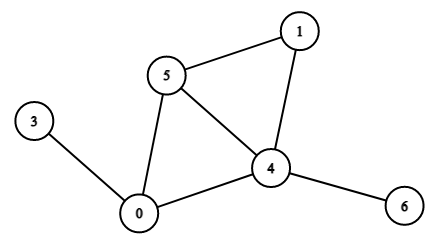
\includegraphics[width=.7\linewidth]{geod.png}
	\caption{A simple graph of 6 vertices and 7 edges. Vertices $v_1$ and $v_3$ have two geodesics meaning that the central vertices are $v_4$ and $v_5$ who share partial control but $v_0$ has full control and is most central between $v_1$ and $v_3$. Note that $v_3$ and $v_6$ cannot be central as they only have one edge each and they only have one geodesic because if $v_5$ or $v_1$ is included then it is no longer the shortest path between $v_3$ and $v_6$.}
	\label{fig:geodesics}
\end{figure}

If there is more than one geodesic, then they are considered to have equal probability in deciding which one to be used. This is simply given by $1/g_{ij}$ where $g_{ij}$ is the number of geodesics between vertices $v_i$ and $v_j$. The formalisation of partial betweenness $b_{ij}(v_k)$ is defined using the idea of geodesics, so for a vertex $v_k$ in $G$ and a vertex pair $v_i$ and $v_j$, the partial betweenness for $v_k$ can be calculated based on the vertex pair and is given by Equation \ref{eq:gb}.

\begin{equation} \label{eq:gb}
b_{ij}(v_k) = \frac{1}{g_{ij}}(g_{ij}(v_k)) = \frac{g_{ij}(v_k)}{g_{ij}} (i \ne j \ne k)
\end{equation}

where $g_{ij}(v_k)$ is the number of geodesics connecting vertices $v_i$ and $v_j$ that include $v_k$ in its path. This essentially translates to the probability that the geodesic chosen for $v_i$ and $v_j$ contains $v_k$. Additionally, notice that $b_{ij}(v_k) = 0$ if there does not exist a path between the vertex pair, $v_i$ and $v_j$ using $v_k$.
This equation can be extended to calculate the betweenness centrality of each vertex. So, for a graph of size $n$, the betweenness centrality value for a vertex $v_k \in V$ is be defined by Equation \ref{eq:cdvk}.

\begin{equation}\label{eq:cdvk}
C_B(v_k)= \sum_i^n\sum_j^n b_{ij}(v_k)
\end{equation}
where $i < j$. This defines the betweenness centrality for $v_k$ and its value increases depending on the number of geodesics that $v_k$ is a part of. The maximum value \cite{freeman2002centrality} was proved by Freeman using a star graph with the central vertex as $v_k$ as all vertices are reachable if they go through the central vertex. Furthermore, this means there are $n(n-1)/2$ paths between all the unordered pairs of the star graph $S$. With $n-1$ edges connected to the central vertex $v_k$. Thus, the betweenness centrality for $v_k$ in $S$ is

\begin{equation}
C_B(v_k)= \frac{n(n-1)}{2} - (n-1) = \frac{n^2-3n+2}{2}
\end{equation}

And if any new edge is added that does not increase the branches of the star, then a new geodesic would form without $v_k$ causing the betweenness of $v_k$ to fall. Therefore Equation \ref{eq:bcrmv} expresses the betweenness centrality of any vertex in a graph $G$ by its representation through a ratio with the maximal value as shown using the star graph S.

Directed edges are required in lexical analysis so we study the use of betweenness centrality and its equations for directed graphs as well.

\begin{equation}\label{eq:bcrmv}
C'_B(v_k)= \frac{2C_B(v_k)}{n^2-3n+2}
\end{equation}

\subsection{Generalisation to directed graphs}
The key idea of betweenness centrality is to evaluate the graph and produce values based on the shortest paths of all the possible pairs of the graph. The higher the betweenness value, the more likely the vertex is on the shortest paths of any two vertices. As this concept investigates the vertices on shortest paths, weighted edges would not benefit this graph evaluation as weights could cause a pair of vertices to be seen as further apart than they are within the graph. Also, for experimentations done later with word graphs, the calculations for betweenness will benefit on edges without weights. As the weights may influence the paths of edges between words when the words have a strict order within a sentence. Nonetheless a brief overview of weight inclusion is given.

In the experimentations of social networks \cite{freeman1979centrality}, the centrality values are used on undirected graphs however an idea to generalise the betweenness to weighted graphs is to take the weights as indication of the distance of the vertices. Meaning that the geodesics of any pair will be defined on the smallest total value of paths between them rather than the shortest path length as shown on Figure \ref{fig:dbc}.

\begin{figure}[!htb]
	\centering
	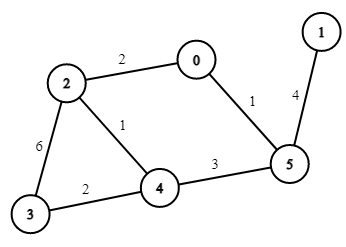
\includegraphics[width=.7\linewidth]{weightedbetween.png}
	\caption{Shows a simple weighted graph. The path between vertex $v_0$ and $v_3$ has 1 geodesic but when considering the weights, this geodesic has a weight of 6. The smallest weighted geodesic is using the path $v_0v_2v_4v_3$ with a weight of 5 instead of the original geodesic. }
	\label{fig:dbc}
\end{figure}

Since weighted edges do not benefit the word graphs when considering centrality, we discuss the generalisation in this section only to directed graphs. If the graph has weights, then they are not implemented to ensure betweenness values will not be influenced and remain congruent throughout experimentation. The geodesic proportions of paths from $v_i$ and $v_j$ was defined earlier in Equation \ref{eq:gb}. Consequently, this equation can be utilised to define pair-dependency of vertices $v_i$ to $v_k$ where the vertex $v_i$ must depend on vertex $v_k$ in order to get to other vertices such as $v_j$ on its geodesics. In other words, $v_k$ acts like a gatekeeper to $v_i$. Therefore, for a graph with $n$ vertices, the pair dependency is defined to be 

\begin{equation}\label{eq:bcrmv}
d^*_{ik} = \sum_{j=1}^{n}b_{ij}(v_k)
\end{equation}

where $i \ne j \ne k$. Matrices can be used to store the pair-dependency values to provide an ease of use and a better representation for all values. The results can be arranged into the matrix $D$ defined as $D = (d^*_{ik})$. The elements of the matrix measures how much the vertex $x$ (corresponding to the row number) depends on vertex $y$ (corresponding to the column number) to connect to other vertices in the graph. Additionally, the betweenness centrality can also be calculated based on this matrix $D$ through the summation of the columns in which the sum will give the betweenness centrality for the column number that represents the vertex. Otherwise shown as

\begin{equation}
\sum_{i=1}^nd^*_{ik} = 2C_B(v_k)
\end{equation}

Which means that the betweenness centrality of $v_k$ is double of the pair dependency column sum \cite{white1994betweenness}. This is because for an undirected graph, the upper and lower diagonal matrix are equal due to the symmetry of graph $G$. The generalisation for directed graph can then be shown to be

\begin{equation}
C_B(v_k) = \sum_{i=1}^nd^*_{ik}
\end{equation}

Therefore, we are able to use the directed version of betweenness centrality to identify centralised vertices of importance. This will be applied to lexical graphs generated by a dataset of under a specified language. We continue to discuss other centrality values that may be of interest.

\subsection{Other centrality values}
Centrality is a larger area within graph theory that is continuously being studied. Other than betweenness centrality, there are other centralities with similar attributes such as the \emph{closeness centrality}, \emph{eigenvalue centrality}, \emph{Katz centrality} \cite{katz1953new} and the \emph{Hyperlink-Induced Topic Search (HITS) centrality}. All of which calculate values for the vertices or edges given their locations amongst their neighbours within the graph by various different methods. Interestingly the closeness centrality can be seen as the duality of betweenness centrality as they can be obtained from row and column summations of the dependency relation defined in the paper by Brandes, Borgatti and Freeman \cite{brandes2016maintaining}.
Betweenness studies the vertices that act as bridges between other geodesics whereas the closeness centrality measures the average distance of the shortest paths between any pairs of vertices. A vertex with high closeness value means that the distance to any other vertex is short on average. 

Closeness centrality \cite{brandes2007centrality} can simply be calculated as the inverse of total shortest distance from a vertex $i$ to all of vertices, demonstrated by equation \ref{eq:cce}.

\begin{equation}\label{eq:cce}
C_C(v_i) = \frac{1}{\sum_{j}^nd(v_i, v_j)}
\end{equation}

where $i \ne j$. This is the calculation is for simply connected graphs however can be easily expanded to directed and weighted graphs. Accomplished by modifying the calculation to use the measure of distances for the graph in question. I.e., take the total weights of the path length rather than the path length for weighted graphs and to consider only correct paths (travelling along an edge in the permitted direction) when investigating directed graphs. Of course, we take the version for directed graphs to be used later in duality of the betweenness centrality. This duality of the centrality values may lead to unique vertex identifications.
\newline

Therefore, by taking these properties, the graph can be rearranged in accordance to their centrality values. This is accomplished by having their property values as their position vector and is done so similarly in the paper by Juan, Alvarez, Villasante and Ruiz-Frau \cite{de2021graph}. In which they relabelled graphs with their normalised centrality values. This ranges from the betweenness centrality to eigenvector centrality. Thus, a similar idea can be applied along with the other properties explained and studied in this chapter.

\section{Webpages}
One of the largest graphs in the modern world is the network of webpages, especially Google's search engine. To help navigate through the vast quantity of pages, Brin and Page \cite{brin1998anatomy} developed an algorithm known as the \emph{Page Rank} algorithm. The Page rank gives a quantified meaning to the importance of the webpages and their links to other webpages. Additionally, the page rank is known as a centrality value which was discussed briefly in the last section along with the Hyperlink-Induced Topic Search (HITS) which was also created with a similar goal to page rank. Both values are based upon digraphs (directed graphs) and were generated to help with the navigation of the world wide web. The algorithms provided users with the highest quality webpages that were also most relevant to their search criteria. The idea of finding the most relevant page can be translated to finding the most relevant word within a sentence. Consequently, we can transfer the values generated for page rank or HITS onto our word graphs later on. In doing so, words of relevance can be found.

In addition to the centrality property, which we use later, we identify a couple web page algorithms and deduce the main one that will be used during lexical analysis. These will either be the HITS algorithm or Page Rank algorithm.

\subsection{Hyperlink-Induced Topic Search}
HITS algorithm calculates the ranks of \emph{authorities} and \emph{hubs} in relation to their in-links and out-links \cite{langville2005survey}. In other words, the edges pointing into vertices and the edges pointing out of the vertices in the graph/network.  Authorities and Hubs are assigned to webpages (vertices) depending on their number of in-links and out-links. For the HITS algorithm, the webpages that have lots of in-links pointing to it are denoted as authorities. The webpages that have lots of out-links pointing to other webpages are denoted as the hubs. These can be identified by the HITS algorithm as the calculations are an iterative process. The iterative process enforces the authorities and hubs by bringing the authorities to the surface of the graph. Leading to the isolation of the authorities and hubs from the other webpages. This is achieved by generating the hub and authority values through mutual reinforcement. Based on vertices $i \in V$ from a graph of webpages $G = (V , E)$, the hub value $h_i$ and authority value $a_i$ are first set to a value of 1. This is so that they are indistinguishable and will later be relabelled if necessary. Then by Kleinberg's HITS algorithm, they are updated iteratively through the formulas:

\begin{equation}
a_i^{(k)} = \sum_{j:j\rightarrow i \text{ \& } j \ne i}h_j^{(k-1)} , \qquad \qquad h_i^{(k)} = \sum_{j:i \rightarrow j \text{ \& } j \ne i}a_j^{(k)}
\end{equation}

where $j$ is denoted as the links from and to the webpages of $i$ and $j$. The $k$ depicts the $k^{\text{th}}$ iteration of the algorithm, so the authority values depend on the previous iteration of hub values and the hubs are calculated based on the current $k^{\text{th}}$ authority values. Which gives the mutual reinforcement of both values. As the graph $G$ can be represented by an adjacency matrix $A = [a_{ij}]$, the formulas can be expressed through matrices \cite{chatzigeorgiou2006application} and vectors instead as shown by Equation \ref{eq:hitsah}.

\begin{equation}\label{eq:hitsah}
\bold{a}^{(k)} = \bold{A}^{T}\bold{h}^{(k-1)} , \qquad \qquad \bold{h}^{(k)} = \bold{A}^{T}\bold{a}^{(k)}
\end{equation}

where the hub and authority values are adapted into vectors $\bold{a}^{(k)}$ and $\bold{h}^{(k)}$. The vectors are expanded and shown as

\begin{equation}
\bold{a}^{(k)} = \begin{bmatrix}
           a_1^{(k)} \\
           a_2^{(k)} \\
           \vdots \\
           a_n^{(k)}
         	\end{bmatrix}
           , \qquad \qquad 
\bold{h}^{(k)} = \begin{bmatrix}
           h_{1}^{(k)} \\
           h_{2}^{(k)} \\
           \vdots \\
           h_{n}^{(k)}
         	\end{bmatrix}
\end{equation}

Accomplishing the goals of generating the values which depict the hubs and authorities more clearly within the graph. Although this algorithm is currently defined only for directed weightless graphs, we extend the algorithm to include a weighted edge version.

As the number of iterations increases, the values generated may increase. This means that at some point, the values will become too large to be used for any calculations. In order to mitigate this problem, the values can be normalised which prevents the issue of tending to infinity. After $k$ iterations, the normalised formulas are demonstrated by Equations \ref{eq:nhits} with the inclusion of weights. The general outline for the HITS algorithm is demonstrated by Agosti and Pretto \cite{agosti2005theoretical} as the following:
\newline

\begin{algorithmic}
\State $\bold{a}^{(0)} := \bold{u}$ ,   $\bold{h}^{(0)} := \bold{u}$;
\For{$k := 1 \text{  to  } K$} 
   		 \State \qquad $\bold{a}^{(k)} = \bold{A}^{T}\bold{h}^{(k-1)}$;
		 \State \qquad $\bold{h}^{(k)} = \bold{A}^{T}\bold{a}^{(k)}$;
		 \State \qquad normalise $\bold{a}^{(k)}$ such that $\norm{\bold{a}^{(k)}} = 1$;
		 \State \qquad normalise $\bold{h}^{(k)}$ such that $\norm{\bold{h}^{(k)}} = 1$;
\EndFor 
\State $\bold{a} := \bold{a}^{(K)}$ ,   $\bold{h} := \bold{h}^{(K)}$;
\newline
\end{algorithmic}

where $K$ denotes the maximum number of iterations and $\bold{u}$ as the vector for the first iteration of hub and authority values, also known as the base case. The base case for $\bold{u}$ will just be the vector of 1s known as $\bold{1}$ or $\bold{e}$ in linear algebra. Then the normalised values after $k$ iterations is given as follows:

\begin{equation} \label{eq:nhits}
\bold{a}^{(k)} = (\bold{A}^{T}\bold{A})^{k-1}\bold{A}^{T}\bold{u} , \qquad \qquad \bold{h}^{(k)} = (\bold{A}\bold{A}^{T})^{k}\bold{u}
\end{equation}

To incorporate weights of the edges into the algorithm, the weighted matrix $W$ for the graph $G$ can be used in place of the adjacency matrix. Simply by replacing the $A$ in the formulas, the weighted version can be generated as the formulas:

\begin{equation} \label{eq:nhits}
\bold{a}^{(k)} = (\bold{W}^{T}\bold{W})^{k-1}\bold{W}^{T}\bold{u} , \qquad \qquad \bold{h}^{(k)} = (\bold{W}\bold{W}^{T})^{k}\bold{u}
\end{equation}

Concluding the study on the HITS algorithm, we now proceed with the Page Rank algorithm which is more commonly known and used.

\subsection{Page Rank}
A widely known algorithm that contributes to internet navigation within Google is the page rank. The page ranks are needed because many different search queries can be entered onto the search engine. These queries produce lots of results that contain the same or similar words to what was searched. Consequently, a method to help organise and prioritise the results is necessary. The page rank is used to rank the webpages according to the number of backlinks a page may have and the number citations that reference a particular page. An example of webpages and links in the form of a graph is shown in Figure \ref{fig:page} with their page ranks displayed. The Page Rank algorithm can also be compared to the HITS algorithm to see the benefits of either. This is explored in the paper by Devi, Gupta and Dixit \cite{devi2014comparative}.

\begin{figure}[!htb]
	\centering
	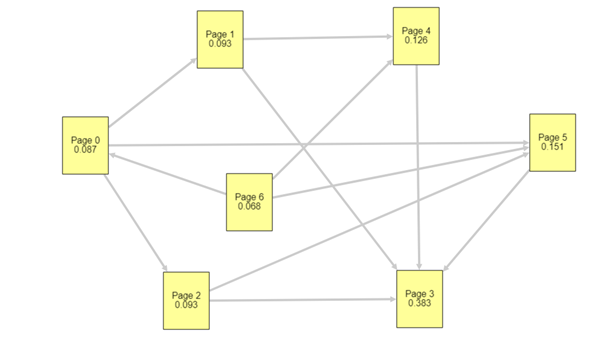
\includegraphics[width=.9\linewidth]{pagegraph.png}
	\caption{A graph representation of webpages and their in and out-links. Algorithms such as Page Rank and HITS use this graph format to help demonstrate their calculations.}
	\label{fig:page}
\end{figure}

For the graph $G = (V, E)$ the webpages can be seen as vertices $v \in V$ with their links as the directed edges between pages, the same way to how they were represented in the HITS formulas. We can let $F_v$ be the set of webpages that $v$ points to, i.e., the forward links. Similarly, the backwards links as $B_v$ which is the set of webpages that points to $v$. The simplified version of Page Rank \cite{page1999pagerank} can then be defined with $N_v = \left|F_v\right|$ in Equation \ref{eq:prb}.

\begin{equation}\label{eq:prb}
PR(v) = c\sum_{w \in B_v}\frac{PR(w)}{N_w}
\end{equation}

where c is a variable used for normalisation purposes so can be modified accordingly. The page rank is calculated by the even distribution of the page rank for webpage $v$ among webpages that $v$ points to. The page ranks that links to other webpages from $v$ are then used to calculate their page rank. Hence giving an iterative approach to calculating their ranks whilst the algorithm travels along the links of the webpages. On the other hand, if a webpage does not have out-links and only in-links from other webpages then their rank is never distributed to others causing its value to accumulate. This situation is known as a \emph{rank sink}.

A remedy to having a rank sink is to use a a damping factor to illustrate the probability that the user follows the links on the webpage. This takes into the consideration that users could skip pages or go directly to another webpage that were not linked through the URL. Hence ($1-d$) is considered as the distribution of the page rank from webpages that were not directly linked to it, i.e., no direct edges between them. Thus ,for the page $v$ with $b_i \in B_v$, the page rank \cite{brin1998anatomy} is defined through Equation \ref{eq:pr}.

\begin{equation} \label{eq:pr}
PR(v) = (1-d) + d (PR(b_1)/F(b_1) + … + PR(b_n)/F(b_n))
\end{equation}

where $F(v)$ was retrieved from the set $F_v$ for the webpage $v$. Page rank is applied to each page and is repeated on further pages until the equation converges. The damping factor adds randomness into the network of webpages so that the rank sink does not occur and ensures the convergence is not reached too quickly. Usually, the damping factor is taken to be $0.85$. 

By using summation, the Page Rank formula can be simply reduced to

\begin{equation}
PR(v) = (1 - d) + d\sum_{w \in B_v}\frac{PR(w)}{N_w}
\end{equation}

The algorithm for calculating page rank can be modified depending on the use and aims. Such modifications include adjusting the vertex and edge values, modifying the damping factor or introducing a new variable into the algorithm. These such changes are known as \emph{personalisation} and an example of personalisation is the \emph{Weighted Page Rank} \cite{xing2004weighted}. Where larger values are assigned to more popular or important webpages rather than the even distribution that occurred beforehand. Webpages that have out-links will instead receive a value proportional to the page's popularity. Their popularity is based off the number of in-links and out-links they hold. These popularity values of the in-links and out-links are represented by $W^{in}_{v,w}$ and $W^{out}_{v,w}$ respectively. $W^{in}_{v,w}$ is calculated by the in-links of webpage $v$, shown to be $I_v$, and the in-links of all the webpages that the webpage $w$ references. This is represented as a set and we call this set of pages $R(w)$ with $I_p$ where $p \in R(w)$. Furthermore with these changes, $W^{in}_{v,w}$ and $W^{out}_{v,w}$ can then be formularised into Equations \ref{eq:prwin} and \ref{eq:prout} respectively.

\begin{equation}\label{eq:prwin}
W^{in}_{v,w} = \frac{I_v}{\sum_{p \in R(w)}}{I_p}
\end{equation}

\begin{equation}\label{eq:prout}
W^{out}_{v,w} = \frac{O_v}{\sum_{p \in R(w)}}{O_p}
\end{equation}

where $O_v$, $O_p$ is defined the same as the in-links previously but with the use of the out-links as a replacement. Therefore, the Page Rank formula can be modified to include the webpage's importance giving us the Equation \ref{eq:proverall}.

\begin{equation}\label{eq:proverall}
PR(v) = (1 - d) + d\sum_{w \in B_v}PR(w)W^{in}_{v,w}W^{out}_{v,w}
\end{equation}

So, this formula is focussed more upon the webpages that are visited more frequently by users and ensures they end up with a higher rank. 

However, for the purpose of general directed weighted graphs, the edge weights are lost in the formula as the algorithm updates the rank of every vertex in each iteration meaning that the weights can be disregarded and replaced with the page ranks instead. To ensure this does not happen, the weights of all the edges must be included in the rank's calculation. This is accomplished by summing up the weight values of the in and out edges and incorporating it into the formula as achieved by Equation \ref{eq:wpr}.

\begin{equation} \label{eq:wpr}
PR(v) = (1-d) + d\sum_{w \in B_v}\frac{PR(w)w_{(w \rightarrow v)}}{N_w}
\end{equation}

where $N_w = \sum_y{A_{w,y}w_{(w \rightarrow y)}}$ is redefined as the sum of weights of the out-linked edges in relation to vertex $w$.
\\

Whilst HITS and Page Ranks are designed for the search engine, the network of webpages essentially is a large directed graph that can contain weights hence why the Page Rank can be used on any derivatives of a weighted directed graph. Thus, these are additional graphical properties that can be used to help analyse the structure and linkage of a graph. 

In conclusion, we take the page rank formulas into the experimentations of lexical analysis. This is because we do not have the requirements of hubs and authorities as shown in the HITS algorithm, so we use the page ranks for directed graphs in future. In addition to the page ranks, we will incorporate the use of local clustering coefficient, trophic levels and the betweenness centrality so that various graph visualisations can be produced. Before applying these to lexical data, we begin with initial experimentations on a smaller dataset shown in the next chapter. This is to ensure that the visualisations work and to implement any modifications that may be required. Also gives us further insight as to what various values represent in a different dataset.


\chapter{Application of Graph Properties}
Now we apply the properties discussed last chapter onto connected graphs to demonstrate their use. These properties are used to outline and modify the graph such that an alternative layout may be given. A different layout means a new visualisation that can reveal correlations between the vertices or edges within the graph. Through the use of Python, I have coded a program to display a graph either generated from a adjacency matrix, a weighted matrix or a data set that is pre-existing. To help accomplish this, I have used Tiago's Graph Tool library for python which contains useful documentation and functions to achieve the graph generations. Along with Tiago's library, I have used other mathematical libraries for complex arithmetic. The general idea is to compare various graph properties by modifying their positions according to the values of their graph properties. For simplicity and the goal of being comparable, we choose the $y$-axis of the graph to be based upon the trophic levels and the $x$-axis to vary between the different properties discussed in the last chapter.

\section{Early Experimentations}
Initially, out of the many pre-existing graphical datasets from Tiago's library, I experimented on a smaller dataset that demonstrates the relationships between karate clubs in a city. This is so that I can test and generate a visualisation of this dataset before lexical analysis. This dataset involves 34 karate clubs where the initial graph can be shown by Figure \ref{fig:karate} with the adjacency matrix in Appendix \ref{app:karateadj}. This is also to test that the visualisations work for a simple undirected graph before using directed graphs. However this means that the trophic levels are not used ideally in this scenario as they focus on directed graphs and their hierarchical structure.

\begin{figure}[!htb]
	\centering
	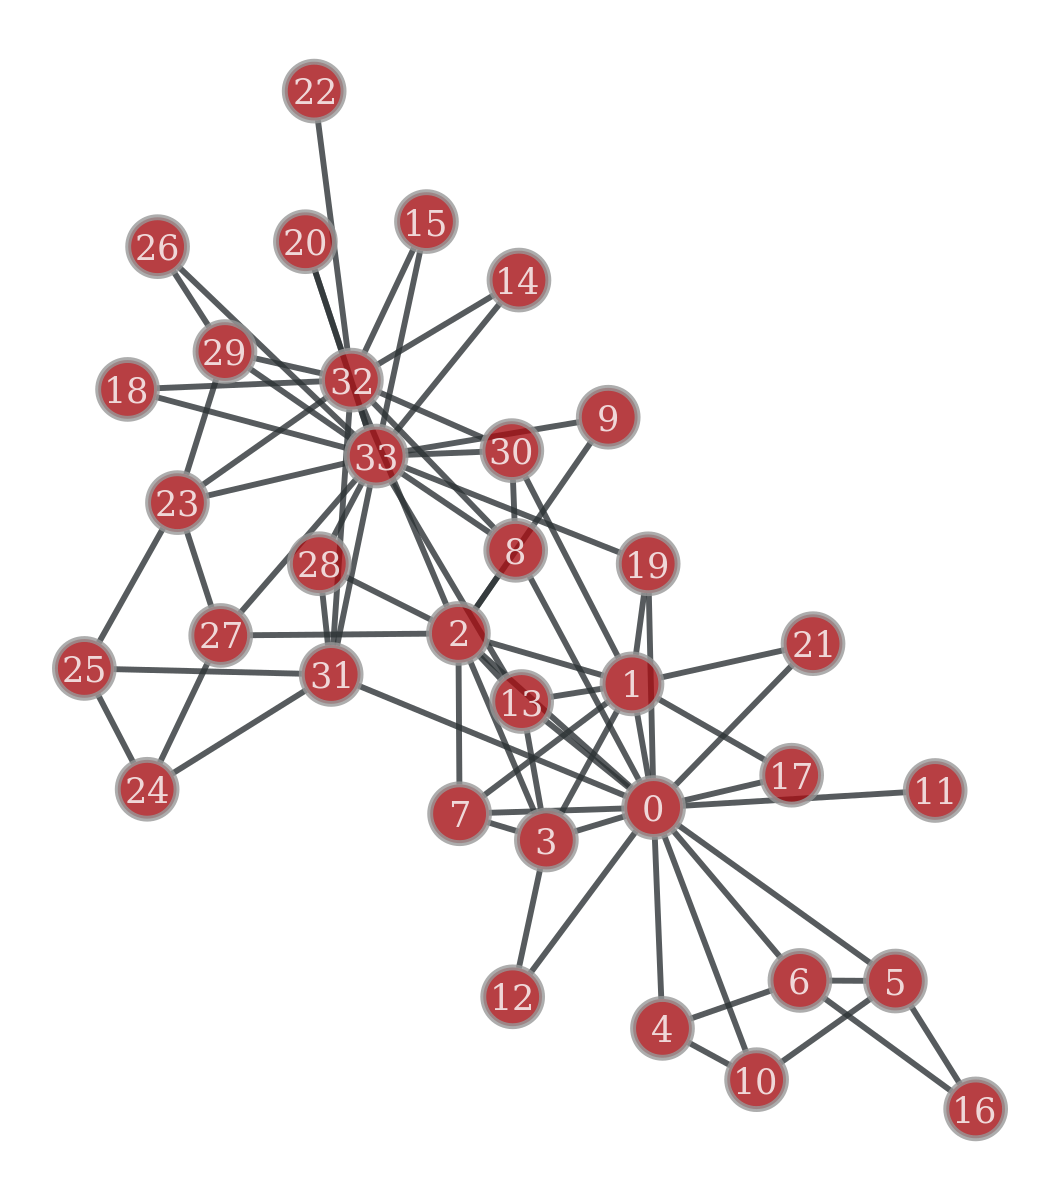
\includegraphics[scale=0.2]{karate.png}
	\caption{The initial graph based on the karate club dataset pre-existing within the library that was generated through the python program. Contains 34 clubs and their connections to one another with no important meaning with the positions of the vertices.}
	\label{fig:karate}
\end{figure}

Current positioning of the graph are determined based on the idea that the vertices do not overlap each other and their connections are easily visible. So the positioning of the elements in the dataset have no real benefits other than having good visibility. Any correlations or vital information can not be derived from the initial graph. The only information that can be derived are the certain outliers who only have one edge, vertices 22 and 11. The vertices that have more edges can also be seen such as vertices 32, 33 and 0 under closer examination. But these vertices are difficult to distinguish at a first glance. Thus, we now include various different graph properties discussed in the last chapter to ensure that more can be visualised. This can be seen in Figures \ref{fig:karatecentrality} and \ref{fig:karatelocal} by using the trophic levels values for each vertex as their $y$-value and another property value for their $x$-value.

For karate clubs, the trophic levels do not represent a clear hierarchical format due to the undirected edges as there is no distinction between ``upstream" or ``downstream" of information. So for vertices such as 1 or 16, they could be recognised as the start or end of the network hence the reason they have the largest and smallest trophic levels. Even if the flow of information is undirected, trophic levels are still useful in implementing some structure into the karate dataset. Further datasets involving languages that will be explored will be directional so that trophic levels can be used optimally.

\begin{figure}[!htb]
\centering
\begin{subfigure}{.45\textwidth}
	\hspace{-2cm}
	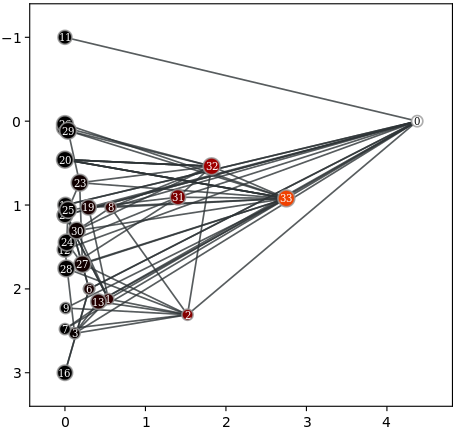
\includegraphics[scale=0.7]{karatebetween.png}
	\caption{}
	\label{fig:karatea}
\end{subfigure}
\begin{subfigure}{.45\textwidth}
	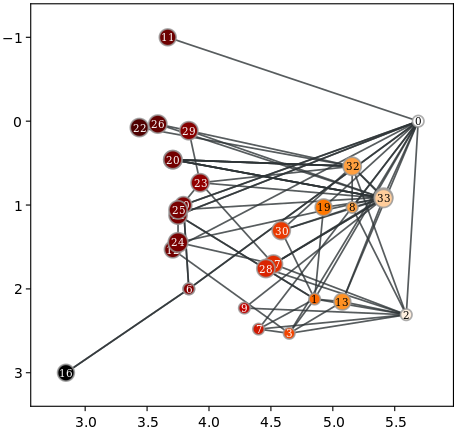
\includegraphics[scale=0.7]{karatecloseness.png}
	\caption{}
	\label{fig:karateb}
\end{subfigure}
\caption{Graph generated by karate dataset, the $y$-axis represents the trophic coherence values and the $x$-axis represents the (a) betweenness centrality values and (b) closeness centrality values for all the vertices. Additionally added colour changes between the $x$-axis to give a clearer visualisation of the separations.}
\label{fig:karatecentrality}
\end{figure}

Figure \ref{fig:karatea} shows the karate graph with the $x$-axis representing the betweenness value. The betweenness value are scaled by a factor of 10 to give a clearer visualisation with betweenness value increasing on the right of the $x$-axis. Which also means the vertex is more frequently involved among short paths of the connections. In this case, the connections of the clubs. We can see that vertex 0 is the furthest vertex on the $x$-axis so is involved in the highest amount of short paths between all the vertices of the karate graph. On the other hand, vertices such as 11, 7, 16, etc, are clubs who are on the outskirts with no convenient connections to other clubs. These vertices are shown to be on the left side of the graph. Therefore, in regards to this dataset, the clubs with larger betweenness are the clubs who are more centralised in a city and have more meaningful links to others.

We compare this to another centrality value, the closeness values which has been scaled by a factor of 10. Figure \ref{fig:karateb} represents this in place of the betweenness value. Through comparison of both, vertices are positioned similarly to betweenness. This is because betweenness are values when considering all vertices within the graph whereas closeness considers all neighbours of a specific vertex. In other words, betweenness measured the control a vertex has over the flow of information through the entire graph, whereas closeness measures the control over the flow of information with vertices in close proximity (i.e., neighbours). Therefore the vertices on the right of both the betweenness and closeness graph would be the most important/largest clubs. Additionally, clubs such as 19 who have a larger closeness compared to betweenness means that it is important to the clubs in close proximity of itself. In other words, the club is the most important/largest within its local area.

\begin{figure}[!htb]
	\centering
	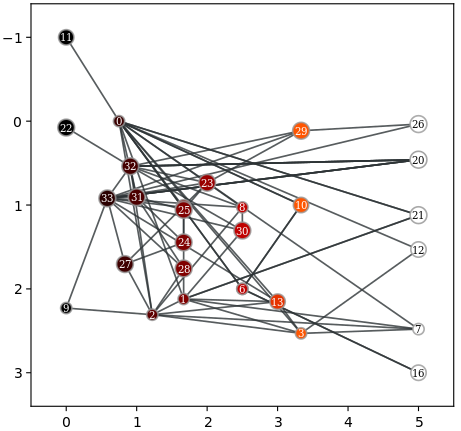
\includegraphics[scale=0.8]{karatelocal.png}
	\caption{Graph generated similarly to the betweenness graph for the karate dataset but the vertices are plotted with local clustering coefficient as the $x$-axis and trophic levels as the $y$-axis.}
	\label{fig:karatelocal}
\end{figure}

Figure \ref{fig:karatelocal} is shown with local clustering coefficient as the $x$-axis instead. Notice that the clubs with less connections to the major clubs (vertices of high degree) are visually seen to the left in both graphs. These vertices would have a low clustering coefficient as well as a low betweenness. On Figure \ref{fig:karatelocal}, the vertices with the best connections to major clubs are located further to the right which are the karate clubs 26, 20, 12, etc. However vertices with high betweenness such as vertex 33 has a smaller local clustering. Due to their club having connections to other smaller clubs, decreasing the overall value of its own connections. So this means that clubs on the right have quicker access or communication with larger clubs and are the closest to them.

All the complex values for each club can be shown in table format, Table \ref{KarateTable}. Apart from the initial column, each column corresponds to one of the different graph property.

\begin{table}[!htb]
    \centering
    \small
    \begin{tabular}{|l|l|l|l|l|}
        \hline
        \textbf{Club} & \textbf{Trophic Levels} & \textbf{Betweenness} & \textbf{Closeness} & \textbf{Local Clustering} \\ \hline
        0 & 0 & 0.437645803 & 0.568965517 & 0.15 \\ \hline
        1 & 2.12094015 & 0.053873557 & 0.485294118 & 0.333333333 \\ \hline
        2 & 2.30804964 & 0.152263709 & 0.559322034 & 0.244444444 \\ \hline
        3 & 2.53039414 & 0.011961881 & 0.464788732 & 0.666666667 \\ \hline
        4 & 1 & 0.000631313 & 0.379310345 & 0.666666667 \\ \hline
        5 & 2 & 0.029987374 & 0.38372093 & 0.5 \\ \hline
        6 & 2 & 0.029987374 & 0.38372093 & 0.5 \\ \hline
        7 & 2.47969196 & 0 & 0.44 & 1 \\ \hline
        8 & 1.02851103 & 0.056737013 & 0.515625 & 0.5 \\ \hline
        9 & 2.22893206 & 0.000847763 & 0.428571429 & 0 \\ \hline
        10 & 1 & 0.000631313 & 0.379310345 & 0.666666667 \\ \hline
        11 & -1 & 0 & 0.366666667 & 0 \\ \hline
        12 & 1.53039414 & 0 & 0.370786517 & 1 \\ \hline
        13 & 2.15210654 & 0.04159151 & 0.507692308 & 0.6 \\ \hline
        14 & 0.45900156 & 0 & 0.370786517 & 1 \\ \hline
        15 & 0.45900156 & 0 & 0.370786517 & 1 \\ \hline
        16 & 3 & 0 & 0.284482759 & 1 \\ \hline
        17 & 1.12094015 & 0 & 0.375 & 1 \\ \hline
        18 & 0.45900156 & 0 & 0.370786517 & 1 \\ \hline
        19 & 1.02788172 & 0.02936057 & 0.492537313 & 0.333333333 \\ \hline
        20 & 0.45900156 & 0 & 0.370786517 & 1 \\ \hline
        21 & 1.12094015 & 0 & 0.375 & 1 \\ \hline
        22 & 0.07623827 & 0 & 0.34375 & 0 \\ \hline
        23 & 0.73415591 & 0.018244949 & 0.392857143 & 0.4 \\ \hline
        24 & 1.44596889 & 0.002209596 & 0.375 & 0.333333333 \\ \hline
        25 & 1.05781988 & 0.003840488 & 0.375 & 0.333333333 \\ \hline
        26 & 0.03492233 & 0 & 0.358695652 & 1 \\ \hline
        27 & 1.70452843 & 0.02170214 & 0.452054795 & 0.166666667 \\ \hline
        28 & 1.75702472 & 0.001794733 & 0.445945946 & 0.333333333 \\ \hline
        29 & 0.1140399 & 0.003869048 & 0.38372093 & 0.666666667 \\ \hline
        30 & 1.30422637 & 0.014727633 & 0.458333333 & 0.5 \\ \hline
        31 & 0.90660502 & 0.140348425 & 0.540983607 & 0.2 \\ \hline
        32 & 0.53811913 & 0.182157888 & 0.515625 & 0.181818182 \\ \hline
        33 & 0.92088243 & 0.275055616 & 0.540983607 & 0.116666667 \\ \hline
    \end{tabular}
	\caption{Table containing all the non-normalised values calculated for each vertex of the graph. The order is in the club number depicted in the first column.}
    \label{KarateTable}
\end{table}

This is the early experimentations of the positioning of vertices within the graph. Instead of using simple datasets, I will generate the datasets based upon various different languages as well as their sentence structure. To understand this further, words in languages must be given a rank to judge their importance. Which can be demonstrated through \emph{Zipf's Law} discussed in the next section.

\section{Zipf's Law}
Zipf's law analyses the natural languages and the frequency of words that appear in them. Alternatively, Zipf's Law \cite{hosch2009zipf} is generally seen as the frequencies of specific events are inversely proportional to their rank that is determined through this law. The law was proposed by George Kinbgsley Zipf when researching the various frequencies of words within the English language. The law states that the $r^{\text{th}}$ most frequent word in the language has a frequency of $f(r)$ which has a relation with the inverse of $r$. Denoting $r$ as the \emph{frequency rank} for the word and $f(r)$ as the frequency of the word in the corpus examined (The \emph{corpus} means the collection of written text).

\begin{equation}\label{eq:zipfs}
f(r) \propto \frac{1}{r^{\alpha}}
\end{equation}

This is the scale for $\alpha \approx 1$ and means that the most frequent word in the examined text which is $r = 1$ has its frequency of appearance to 1, the next most frequent word which is $r = 2$ has a frequency appearance of $\frac{1}{2^{\alpha}}$ and so on. Zipf's law can be drawn on a graph to show a relation and when $log(f)$ is drawn against $log(r)$, the graph generates a curve that closely resembles a straight line with a slope of $-1$. This is known as Zipf's curve and later in the 1960s, the curve's nature was reinforced by the law being correct for smaller \emph{corpora} (the plural of corpus) \cite{sicilia2002extension}. However the curve varies depending on the corpora as expected and the higher ranking words deviated more from the straight line. Therefore, Mandelbrot derived a generalisation for Zipf's law to adjust to the frequency distributions within the different languages. Mandelbrot proposed to adjust the rank by a constant $\beta$, demonstrated by

\begin{equation}\label{eq:zipfs}
f(r) \propto \frac{1}{(r + \beta)^{\alpha}}
\end{equation}

Generalisation of Zipf's law can then be applied to various different corpora of languages so that a frequency distribution can be viewed for the corpus. An example of this can be seen in Figure \ref{fig:zipfwiki}.

\begin{figure}[!htb]
	\centering
	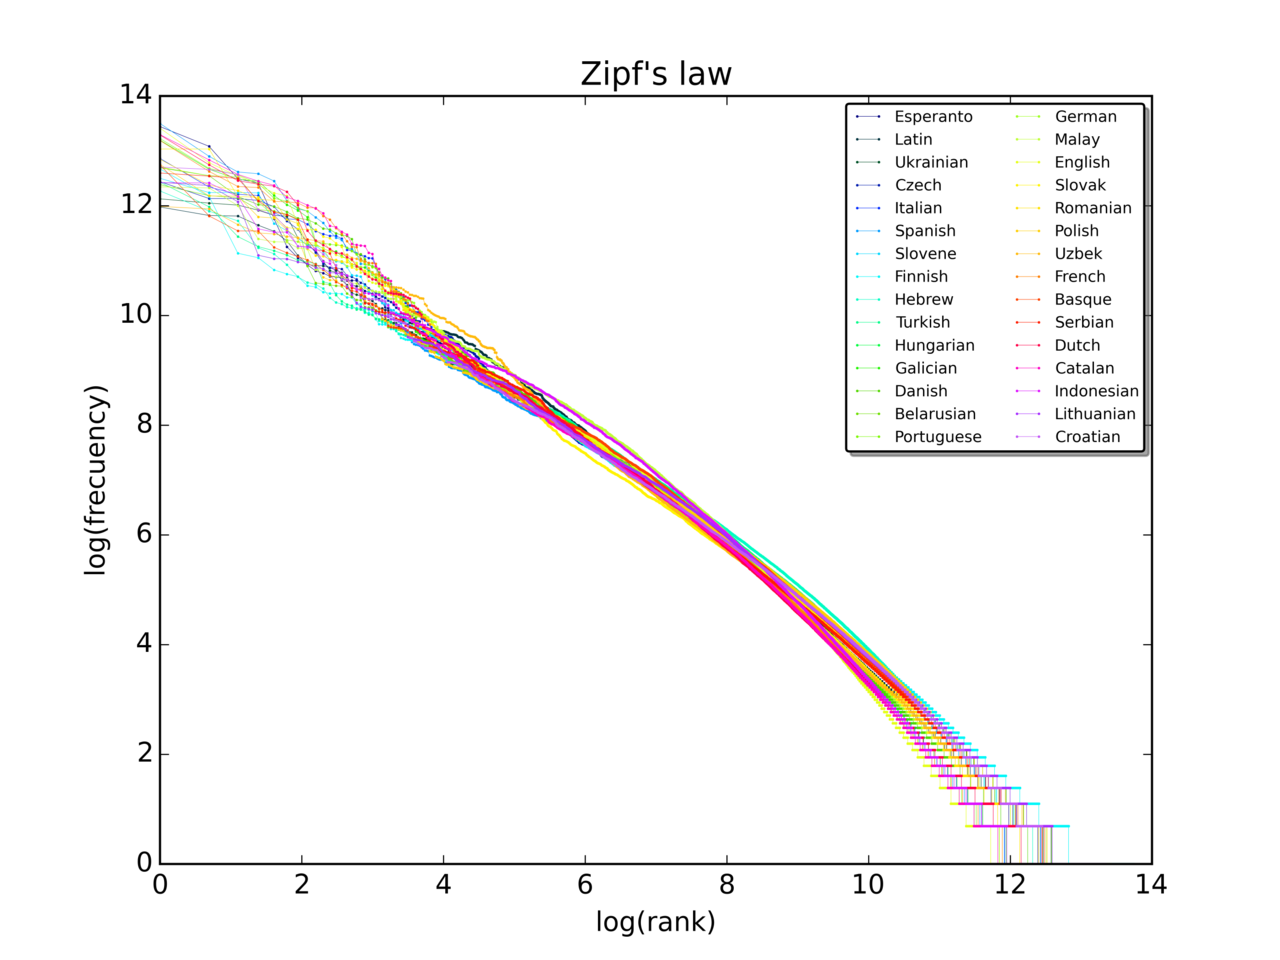
\includegraphics[scale=2.5]{zipfwiki.png}
	\caption{The plot of Zipf's law containing 30 different language corpus generated from the first 10 million words in each language from Wikipedias. The image was sourced from Wikipedia \cite{zipffigure}. }
	\label{fig:zipfwiki}
\end{figure}

So words in a corpus has a systematic relationship between their rank in their occurrence table. Meaning that they are the words most commonly used such as ``the", ``or", ``of". These words account for most of the word occurrences in the English language. Other words such as ``xylophone" and ``accordion" have the least occurrence in English. A larger corpus is studied by Bentz, Kiela, Hill and Buttery \cite{BentzKielaHillButtery} where they study Zipf's law for Old English and Modern English. They study the frequency and ranks of each word whilst comparing them between the old and new English. In doing so, for old English, the words ``and" is ranked first with a frequency of 1731 whereas in modern English, ``the" is ranked first with a frequency of 1775 and ``and" is second instead with a frequency of 1024. By looking at more words and the comparisons between them, old English has a larger number of distinct words whilst modern English has less. However, modern English has a higher frequency for its first 100 words.

In conclusion Zipf's Law is a useful tool because languages tend to follow Zipf's curve in terms of their frequencies and rank. Consequently, by following an existing corpus of language, the data can be extrapolated and used in other corpora to determine similarities between the known and the unknown texts. As well as to use it to determine the types of words that are deemed to be most common in a language.

\chapter{Analysing Languages}
Learning from prior graph generations of each complex property in the last chapter, adjustments have been made for improvement in analysis. This includes normalisation values calculated into a range of 0-10 instead of a simple scale factor. In doing so, ensures that graphs have the same size and axis ranges to provide easier visual comparison. Additionally, I have included page rank in the properties that are studied which were trophic levels, betweenness centrality, closeness centrality and local clustering coefficients. Finally the lexical datasets I will use will be generated through my program by an input of text. Afterwards will be converted into graphs where the words represent the vertices and the edges are directed to the next word in the order of the text. A factor that affected the dataset was the punctuation so to achieve congruent data, the punctuation are stripped unless they symbolises the end of a sentence such as full stops, question marks, exclamation marks etc. Therefore, the graphs we experiment on are directed graphs generated from different language families.

\section{Linguistics}
Modern languages are descendants of ancestral languages through evolution of linguistics. Throughout the different ages of the world, language have been a key part in communication between societies. They are developed and taught to newer generations to reach the stages in the current world. The history of languages can be viewed as a family tree where modern languages are nearer the bottom. Within this trees, there are groups of languages that will share a common ancestor. These are defined to be the \emph{language family} of the languages branching off it.

Estimations of around 500 language families exist and Campbell \cite{campbell2018many} has reported that there are exactly 406 independent language families including dead languages and \emph{language isolates} (where the language does not fit into any language family). According to Ethnologue \cite{eberhard2023a}, who are the research centre for language intelligence, there are 142 different living language families. Of the living families, six are considered to be the major families. These families are known as the Indo-European, Afro-Asioatic, Niger-Congo, Austronesian, Sino-Tibetan and Trans-New Guinea.

The aim of my research is to study modern languages that fall under the Indo-European language family and the Sino-Tibetan language family. \emph{Proto-languages} are alternative names for major language families since they are the parent language to many other languages \cite{rowe2022concise}. English, German and Dutch are Germanic languages under the Indo-European language family. Russian and Polish are Balto-Slavic languages under the Indo-European family.  French and Spanish are Latin languages under the same language family. Chinese falls under a different language family, the Sino-Tibetan family. Furthermore, I will also look at Japanese which is part of the Japonic family but would have been considered a language isolate if the Ryūkyūan languages were not distinct from Japanese \cite{campbell2010language}. Therefore all the languages mentioned will be used in translating the chosen text extract into their relative datasets.

\section{Text Corpus}
The best way in comparing the results to other languages is to have datasets based on the same text extract. Thus, the text extract chosen should be simple and well know. In my case, I have chosen to use the popular story in many languages known as ``Sleeping Beauty". To ensure that the same version is used, the Grimm Brothers version is utilised where the original was in German and extracted from the book of children stories ``Kinder- und Hausmärchen" \cite{grimm1857kinder}. So using translations of this story, word graphs will be generated and experimented on.  Additionally, instead of using the entirety of the story, the first two paragraphs are used so that the graphs are not overwhelmingly dense whilst maintaining any key attributes in the various languages. A partial extract of the first two paragraphs is given as follows (the full two paragraphs is shown in Appendix \ref{textcorpus}):
\begin{quote}
``In times past there lived a king and queen, who said to each other every day of their lives, ``Would that we had a child!" and yet they had none. \dots There were thirteen of them in his kingdom, but as he had only provided twelve golden plates for them to eat from, one of them had to be left out."
\end{quote}
In conclusion the nine datasets are created based on this text extract for graph property calculations. In the next section, the study of Indo-European languages will be undertaken, beginning with English.

\section{Indo-European Language Family}
Five languages of the Indo-European language family were analysed but detailed analysis of English, German and French will be given in this section. Throughout the analysis, words are referred to as vertices and vice versa. The two paragraph extract of "Sleeping Beauty" will simply be referred to as the story corpus of it's relative language. Edges of the generated graph will represents the connections to the subsequent word in the story corpus. 

Before the analysis can be undertaken, a brief summary of the languages structure and grammar is given. This is to ensure the increased understanding of correlations and results achieved through this process.

\subsection{English}
English words can be organised into eight different \emph{parts of speech}; Nouns, Pronouns, Adjectives, Adverbs, Verbs, Prepositions, Determiners and Conjunctions. Linguistic researchers focus on the use of these categories in different situations such as through speaking or in magazines \cite{khaisaeng2017study}. We will study the appearances of these categories in our story corpus. To achieve this, the English story corpus is converted to a dataset so that a directed graph can be generated shown in Figure \ref{fig:engword}. Additionally, in replacement of having each vertex labelled by the corresponding word, each vertex will be labelled with an integer shown in Figure \ref{fig:engnum}. The corresponding integer for each word will be shown on the table of values for the graph. The entire table can be seen in Appendix \ref{app:engtable} while holds 99 unique words.

\begin{figure}[H]
\centering
\begin{subfigure}{.45\textwidth}
	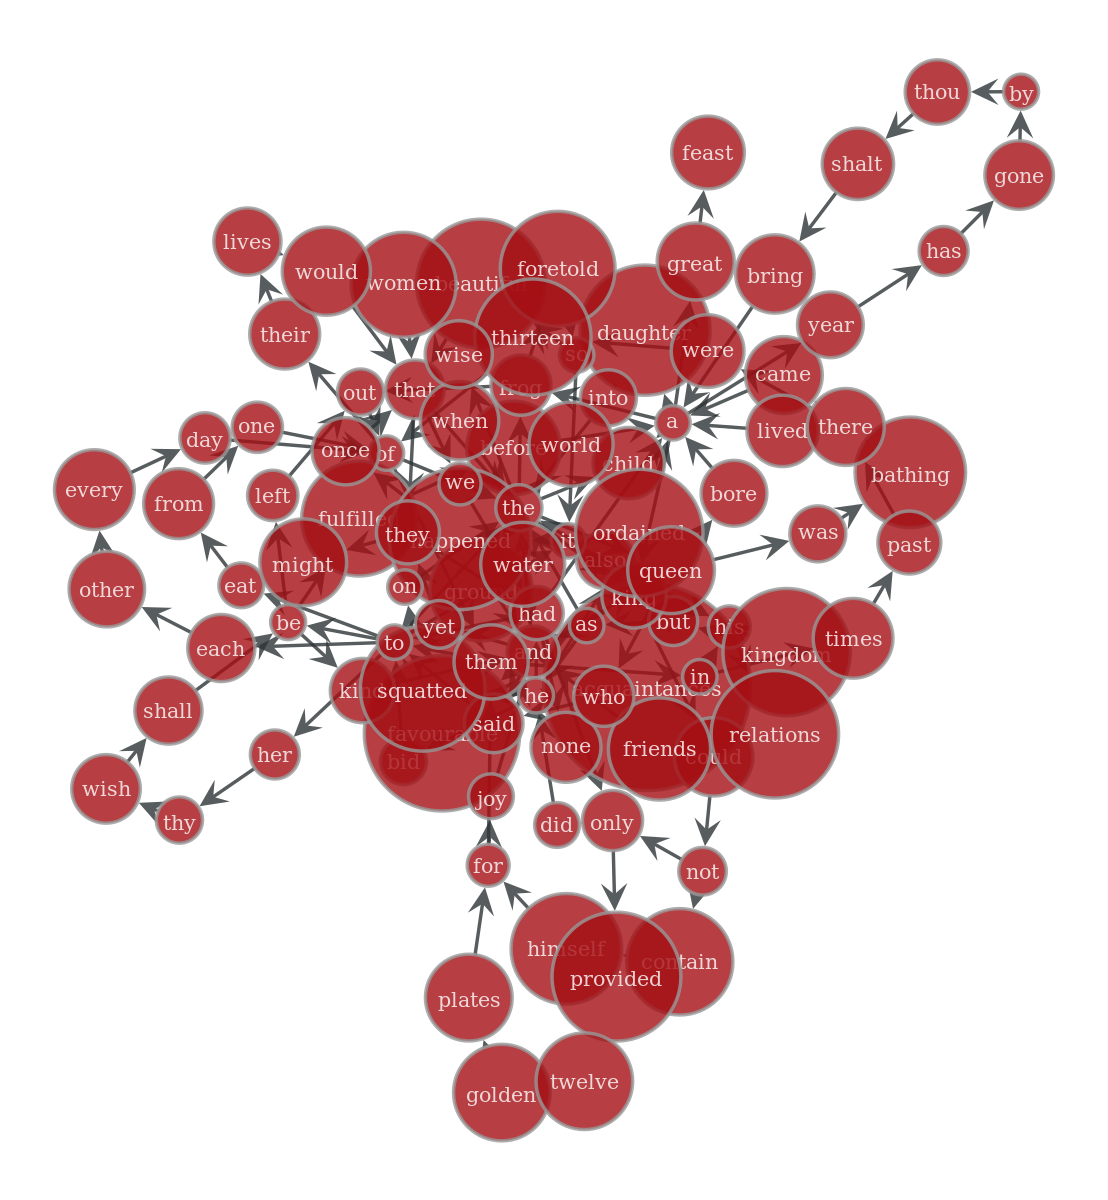
\includegraphics[scale=0.2]{englishwordgraph.png}
	\caption{}
	\label{fig:engword}
\end{subfigure}
\hfill
\begin{subfigure}{.45\textwidth}
	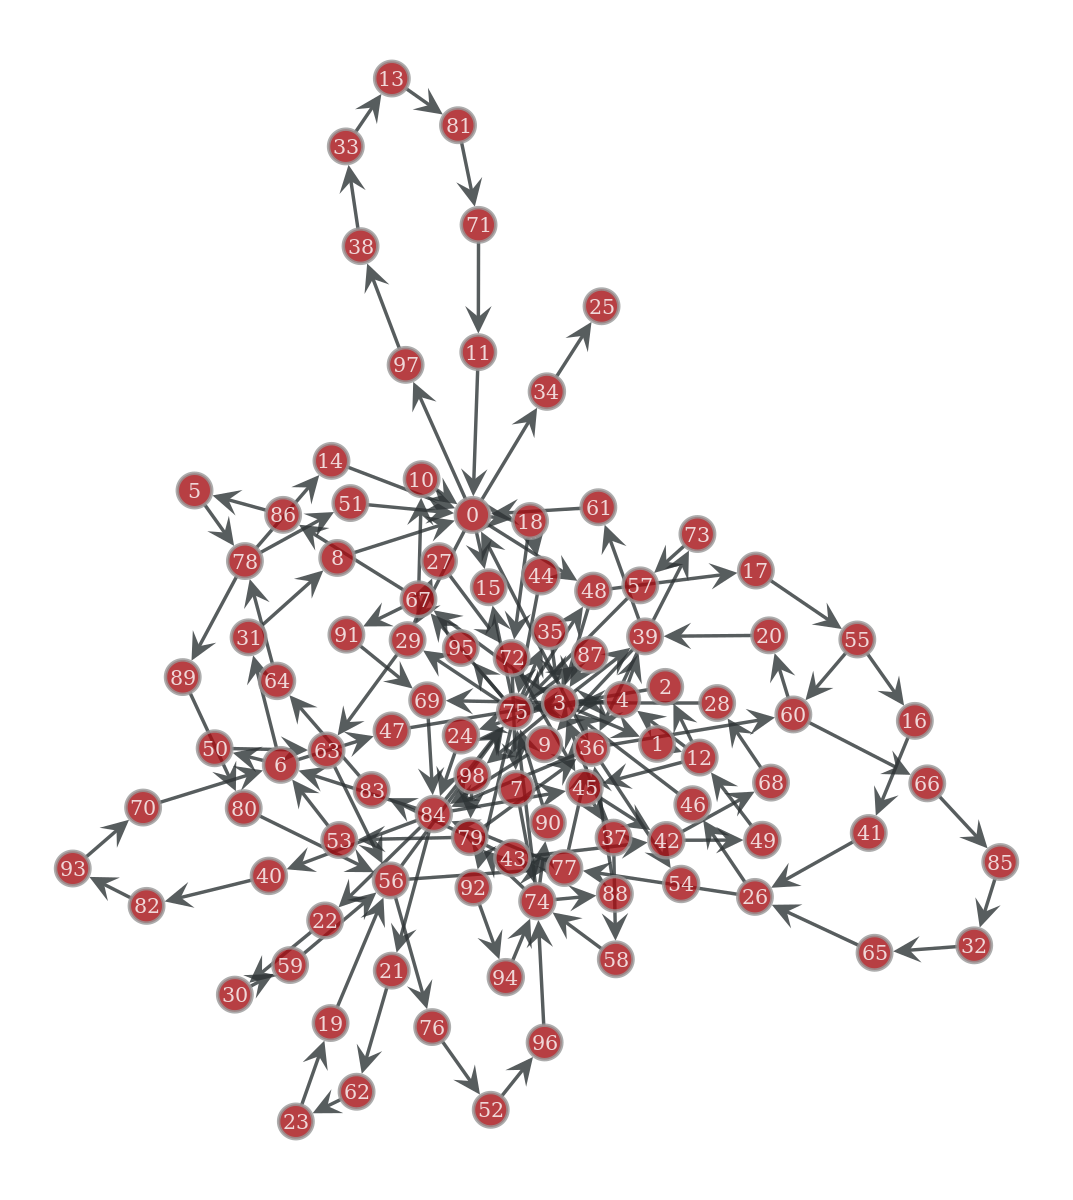
\includegraphics[scale=0.2]{englishnumbergraph.png}
	\caption{}
	\label{fig:engnum}
\end{subfigure}
\caption{Initial graphs generated off the English story corpus. (a) shows the graph with vertex labelling of their corresponding words. (b) shows the same graph but with integer labels rather than word labels to provide better visibility.}
\end{figure}

As done in the Early Experimentations of the karate club dataset, we calculate the values of the various graph properties explained in Chapter 2. These are graph properties such as local clustering coefficient, betweenness centrality, closeness centrality, trophic levels and additionally, page rank. Values are organised into their corresponding columns and presented as a table using abbreviations of each graph property. For example, ``TL" for trophic levels, ``CC" for closeness centrality, etc. The ten most frequently used words are shown in Table \ref{table:englishtop} below. Where the count denotes the frequency of the words appearance in the English story corpus. 

\begin{table}[H]
\centering
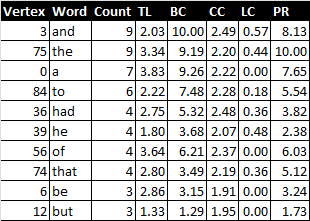
\includegraphics[scale=1]{englishtabletop10.png}
\caption{The first 10 most common words of the dataset. Generated from the English version of ``Sleeping Beauty" in a table format.}
\label{table:englishtop}
\end{table}

We begin by analysing words with the most recurrences (see Table \ref{table:englishtop}). In the order of most frequent to least, the words are ``and'', ``the", ``a", ``to", ``had", ``he", ``of", ``that", ``be" and ``but". Note that nouns, adverbs and adjectives do not appear in the most frequent words. These are the words that are deemed more vital in the creation of structure within a sentence of the story corpus. Any sentence in ``Sleeping Beauty" will have a high chance of containing at least one of these words. Since this is only a portion of a dataset, we can compare these words to a larger dataset to see whether or not the importance of these words remain same. Word frequencies follow the Zipf curve for languages, as discussed in the previous section, so we can take another corpus to compare its frequency of words to ours. We choose to compare the story corpus to the British National Corpus (BNC) \cite{bnc2007british} which is a 100 million word collection that includes both written and spoken English language. The benefits in choosing BNC is that it contains older English so may provide clearer correlations to the story of ``Sleeping Beauty" (the Brothers Grimm version began in the late 18th century). So for the BNC, the top ten words \cite{leech2014word} in order of frequencies are ``the", ``of", ``and", ``a", ``in", ``to", ``it", ``is", ``to" and ``was". Comparing the most frequent words in both corpuses, correlations are achieved such as the repetitions of words ``the", ``to", etc. Such similarities reinforce the fact that the English language has a structured form that requires the use of these such words, as demonstrated with a much smaller corpus compared to the the BNC.

\begin{table}[H]
\centering
\begin{subtable}{.45\textwidth}
	\centering
	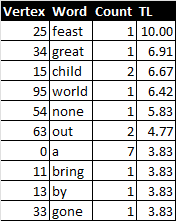
\includegraphics[scale=1]{engtabletctop.png}
	\caption{}
	\label{table:englishtoptc}
\end{subtable}
\hfill
\begin{subtable}{.45\textwidth}
	\centering
	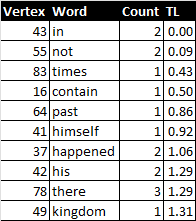
\includegraphics[scale=1]{engtabletcbot.png}
	\caption{}
	\label{table:englishbottc}
\end{subtable}
\caption{Partial extracts of the table data ordered by their trophic levels. (a) Top 10 words ranked by their trophic levels based on the English Story Corpus. (b) Bottom 10 words ranked by their trophic levels based on the English Story Corpus.}
\end{table}

Now onto the analysis of Trophic levels and coherence (see Tables \ref{table:englishtoptc} and \ref{table:englishbottc}). When applying trophic level calculations on directed word graphs, the levels represent the positioning of the word within its relative sentence. Similarly shown in the analysis of network data in empirically-derived directed networks \cite{johnson2017looplessness}. For the "Sleeping Beauty" English word graph, the lower trophic levels denotes the vertices most likely to be sentence starters and the higher levels denote the sentence enders. This is supported by the data because the top six words with largest trophic levels values (ranging from 10.00-4.77) are all sentence enders or accompanied a sentence ender (vertex 34). Along with the bottom five being words (trophic values ranging from 0.00-0.86) nearer the start of sentences such as "there" and "times" in relation to the corpus. However trophic incoherence is calculated to be 0.91 which means that the levels in the graph can not be distinguished and are not clear. Since the $\text{trophic coherence} = 1 - \text{trophic incoherence} = 0.09$ which is due to the fact of the vast difference of sentence lengths in the corpus. Which varies from the shortest sentence of five words and the longest of forty seven words. Consequently in relation to the extract used, a clear hierarchical layout may not be provided but there remains a good layout for sentence flow. Demonstrated by further graphs with the trophic levels as the y-axis ranging from 0 at the top to 10 at the bottom to provide a normal cascade of words. Further graphs includes other graphical properties starting with betweenness and closeness centrality (Figures \ref{fig:engbc} and \ref{fig:engcc}).

\begin{table}[H]
\centering
\begin{subtable}{.2\textwidth}
	\centering
	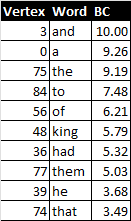
\includegraphics[scale=0.9]{englishtablebc.png}
	\caption{}
	\label{table:englishtablebc}
\end{subtable}
\hfill
\begin{subtable}{.2\textwidth}
	\centering
	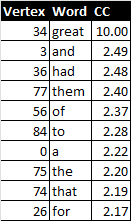
\includegraphics[scale=0.9]{englishtablecc.png}
	\caption{}
	\label{table:englishtablecc}
\end{subtable}
\hfill
\begin{subtable}{.2\textwidth}
	\centering
	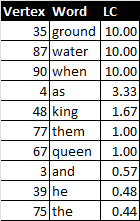
\includegraphics[scale=0.9]{englishtablelc.png}
	\caption{}
	\label{table:englishtablelc}
\end{subtable}
\hfill
\begin{subtable}{.2\textwidth}
	\centering
	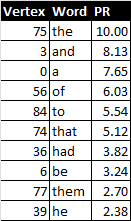
\includegraphics[scale=0.9]{englishtablepr.png}
	\caption{}
	\label{table:englishtablepr}
\end{subtable}
\caption{Partial extracts of the table data ordered by their trophic levels.}
\end{table}

Extraction of the top ten vertices for each graph property to provide ease of comparison later on with the graph visualisations.

\begin{figure}[H]
\centering
\begin{subfigure}{.45\textwidth}
	\hspace{-1cm} 
	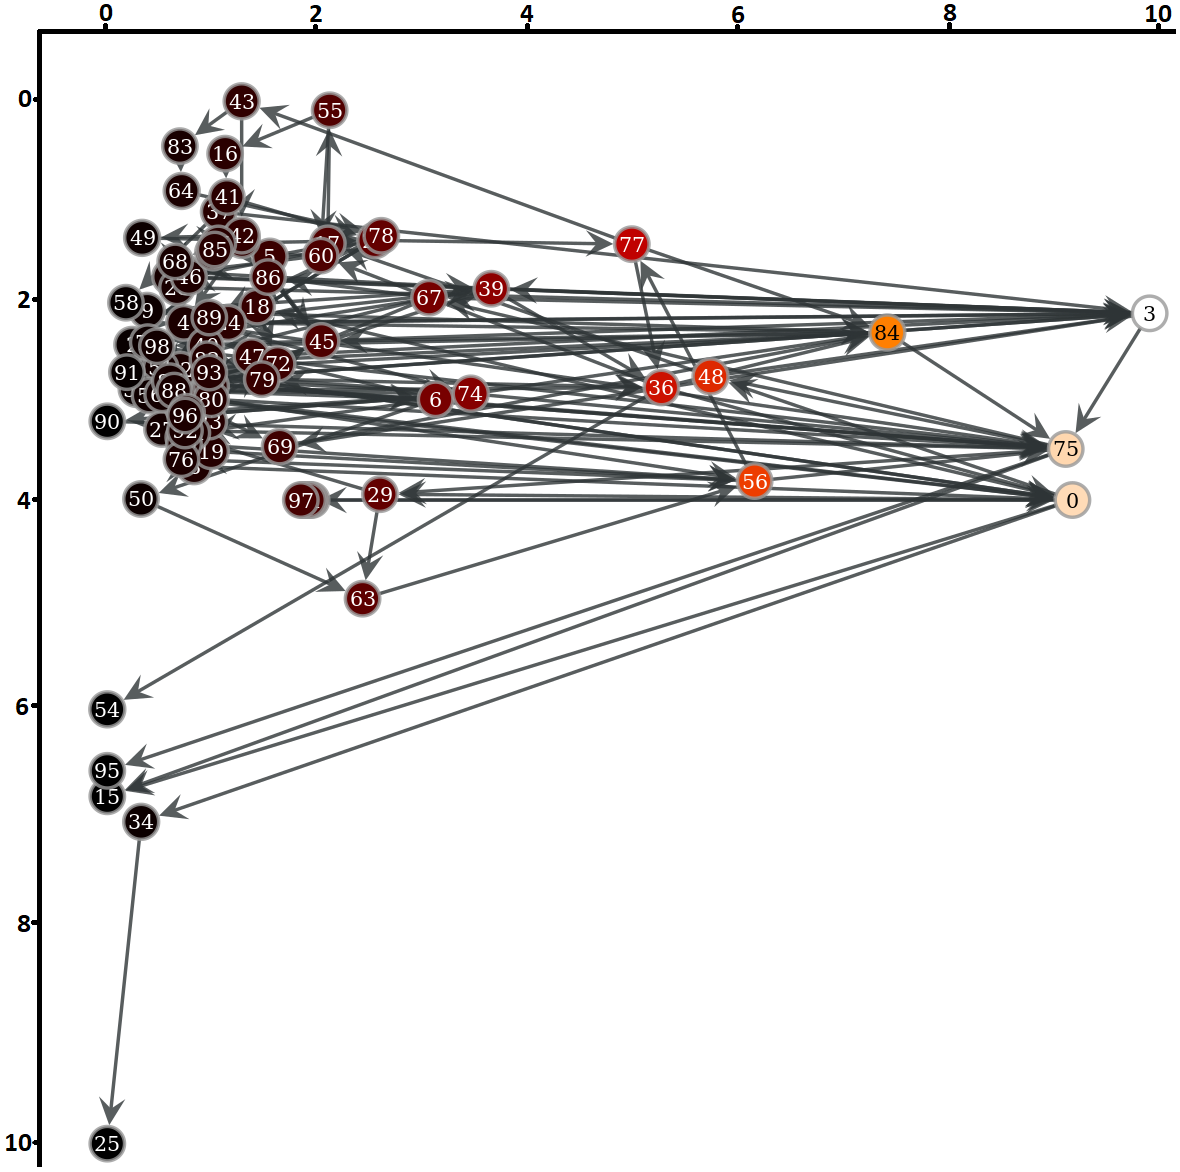
\includegraphics[scale=0.2]{englishbetweenness.png}
	\caption{}
	\label{fig:engbc}
\end{subfigure}
\hfill
\begin{subfigure}{.45\textwidth}
	\hspace{-1cm} 
	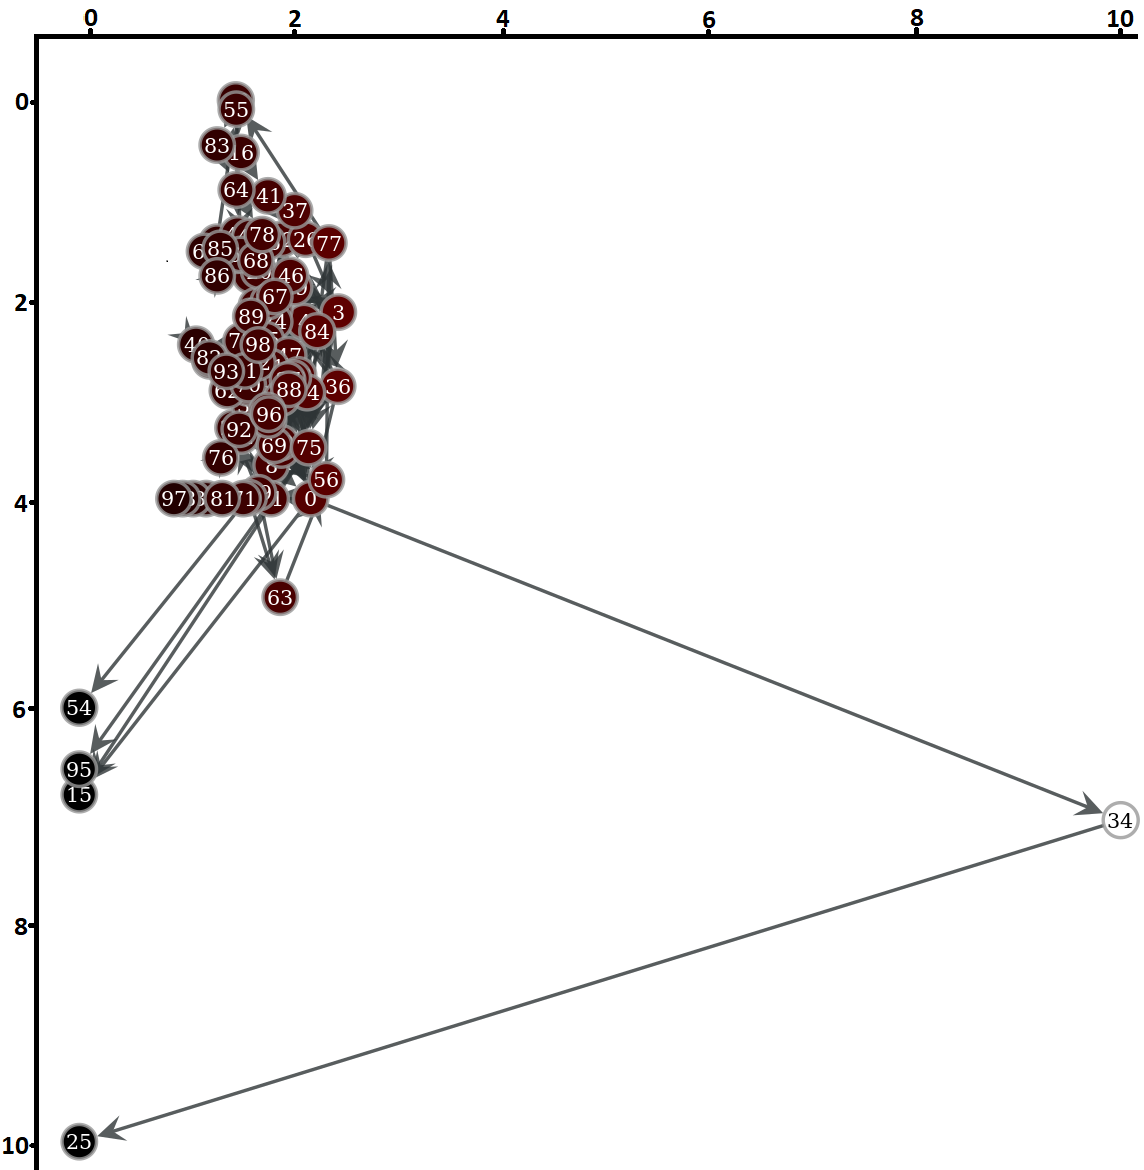
\includegraphics[scale=0.2]{englishcloseness.png}
	\caption{}
	\label{fig:engcc}
\end{subfigure}
\caption{The x-axis positioning of vertices are altered based on their (a) betweenness centrality and (b) closeness centrality values. The y-axis uses the trophic levels.}
\end{figure}

As visually demonstrated on Figures \ref{fig:engbc} and \ref{fig:engcc}, the centrality values for each word is plotted against their trophic levels. Both have been normalised to a range of 0-10 with Figure \ref{fig:engbc} showing the betweenness centrality on the x-axis and Figure \ref{fig:engcc} showing the closeness centrality. The axis are provided here to demonstrate the ranges however will not be included for future graphs because they follow the same axis layout.

Key vertices can be visually identified based on their betweenness values. These vertices are vertex 3, 0 and 75 which are the words ``and", ``a" and ``the" respectively (shown by the Table \ref{table:englishtablebc}). These are conjunctions and determiners of the English language and they have the largest frequency of appearance in the story corpus discussed before. Demonstrating a strong link between the betweenness centrality values of vertices to the word frequencies within the text. Furthermore, these words are common in forming correct structure of a typical English sentence meaning that high betweenness associates the words as key bridges in a sentence. 

When considering closeness centrality, the graph shows that almost all vertices have a similar closeness value in comparison to their betweenness. This is because the closeness centrality analyses the importance of the words within their local clusters rather than the graph as a whole. Meaning that words with high closeness values are key connections in their relative clusters, in other words the sentences that they are part of. However vertex 34 (the word "great") is an outlier and by further analysis, vertex 34 is the only connection between vertex 0 and 25. Also vertex 25 has the highest trophic level and vertex 0 has a low trophic level but a higher degree. Consequently, the closeness value for 34 is an extreme due to the fact that it is the only predecessor of vertex 25. Thus meaning that vertex 34 is the only local bridge in it's sentence giving it an extreme closeness whereas other vertices contains multiple connections.

In conclusion, based on the story corpus, betweenness finds the words most commonly used as connectors in a sentence and closeness finds the words that are likely to isolate later vertices.

\begin{figure}[H]
\centering
\begin{subfigure}{.45\textwidth}
	\hspace{-1cm} 
	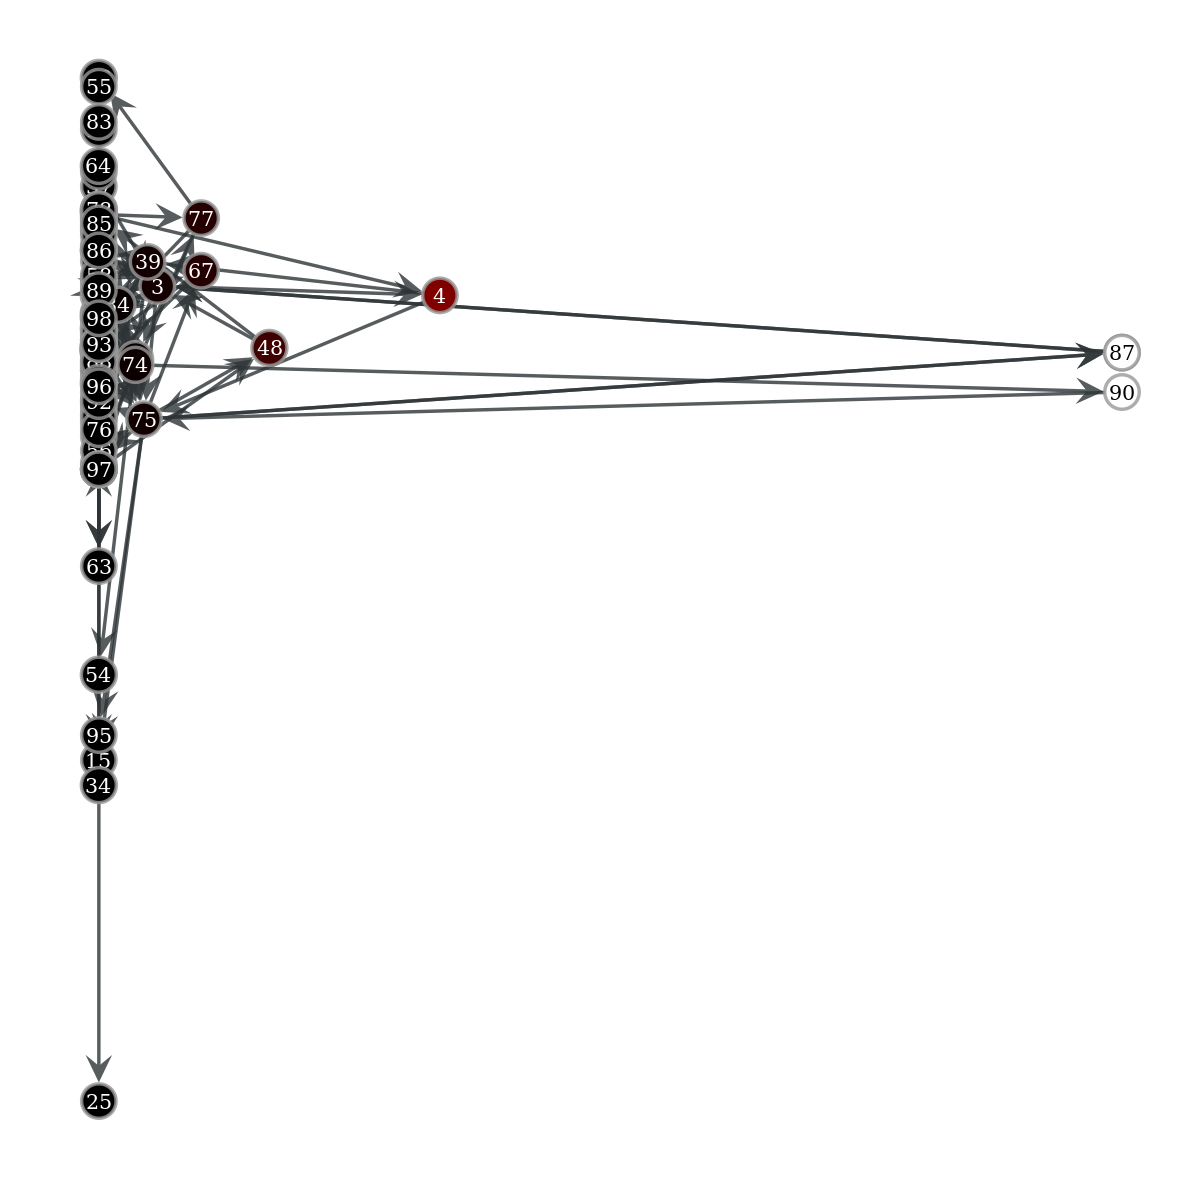
\includegraphics[scale=0.2]{englishlocalclustering.png}
	\caption{}
	\label{fig:englc}
\end{subfigure}
\hfill
\begin{subfigure}{.45\textwidth}
	\hspace{-1cm} 
	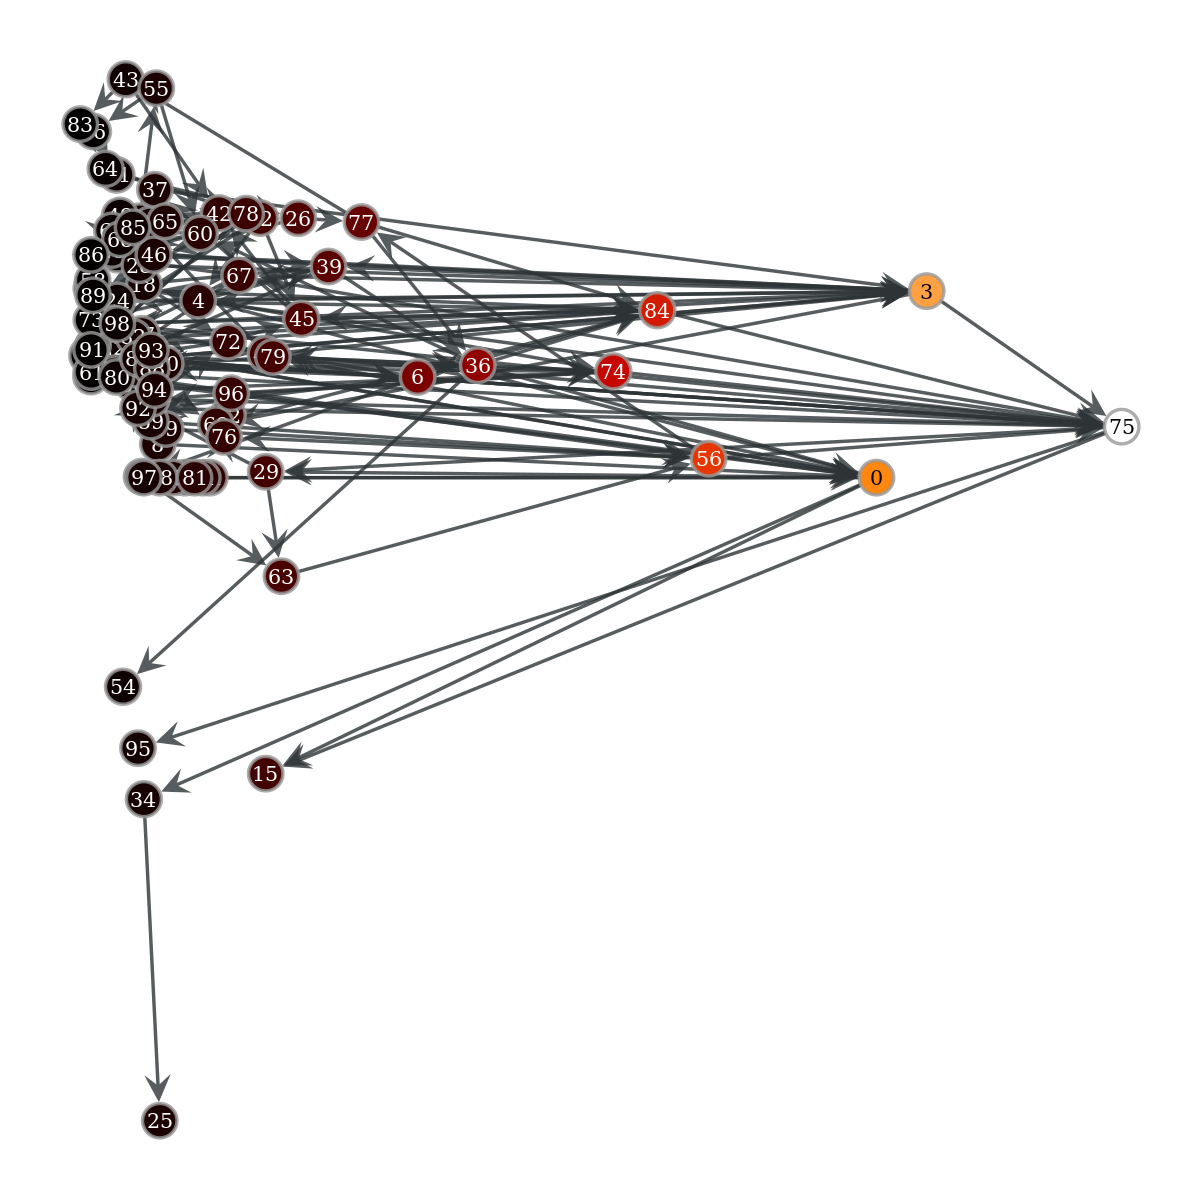
\includegraphics[scale=0.2]{englishpagerank.png}
	\caption{}
	\label{fig:engpr}
\end{subfigure}
\caption{Instead of centrality values like before, (a) local clustering coefficients and (b) page ranks are used for the x-axis. The y values remain the same representing the trophic levels.}
\end{figure}

Finally, local clustering coefficients and page ranks of the vertices within the English word graph are presented similarly as before.  Local clustering coefficients in Figure \ref{fig:englc} and page ranks in Figure \ref{fig:engpr} along with their respective table extracts shown before in Tables \ref{table:englishtablelc} and \ref{table:englishtablepr}. 

Immediately, the local clustering graph shows very few vertices who has a high local clustering, the main ones being vertices 87 and 90 ("water" and "when" respectively). However, there does not exist a clear relationship between these words other than neighbours of these words have have a high degree or importance in the graph. Important words such as ``and" and ``a". On the other hand this is only for the English version of the story so other languages may lead to different results. The page rank of each vertex shows the importance of each word beyond their direct contact. Essentially it has elements of both closeness and betweenness centrality which the graph reinforces since it is visually similar to the betweenness English graph.

In conclusion, when analysing the English language, trophic levels have provided a naturally flow of data presentation from top to bottom in the various graphs generated. Where some sections of the graph are grammatically correct when following their flows. Betweenness centrality and page rank both identified the words of most importance with respects to their neighbours. Closeness centrality also identified words of key importance but at a local level. Finally local clustering coefficients do not provide sufficient benefits when visualising the dataset in the English language. Therefore the results generated based on the English version can be extrapolated to represent the English language. Which is achieved through the identification of the words position in the structure of a sentence and its relative importance. This could also be used for languages that have a similar grammatical structure to English. Now we move onto the analysis of a different translation of the story corpus, German.

\subsection{German}
German is also a Germanic language under the Indo-European language family, same as English. However whilst modern English no longer uses the inflectional case system in grammar, the German language still does\cite{durrell2011hammer}. So as well as the parts of speech in English, German words can be divided into two groups, the words which are \emph{inflectable} and \emph{uninflectable}. If a word is inflectable then their form changes based on the context that the word is used in. These include the three genders for the words (masculine, feminine and neutral), the four cases (nominative, accusative, genitive and dative) and the number (singular or plural). Uninflectable words are known as \emph{modal particles} and mainly used to highlight an emotion of the sentence in spoken language. Therefore the German language is considerably more varied compared to the English language. Meaning that, in theory, the dataset would contain more unique words overall. Which is proven to be true as the dataset based on the story corpus for German contains 109 words whilst English had only 99.

Expectations of the graph properties for the German language is that there would be more unique words of higher importance based on the different genders for words and particles. Word graphs for the German version of the story corpus are generated and shown in Figure \ref{fig:gergraph}. Similarly as before, each number references the same word in it's position.

\begin{figure}[H]
\centering
\begin{subfigure}{.45\textwidth}
	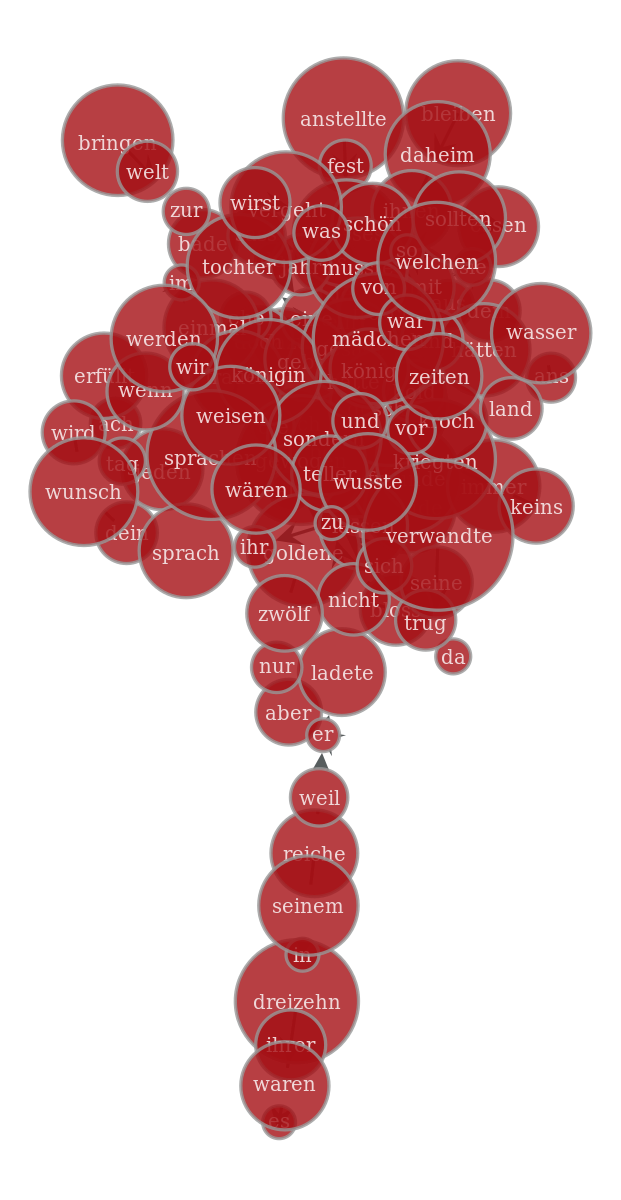
\includegraphics[scale=0.3]{germanwordgraph.png}
	\caption{}
	\label{fig:gerword}
\end{subfigure}
\hfill
\begin{subfigure}{.45\textwidth}
	\hspace{-2cm} 
	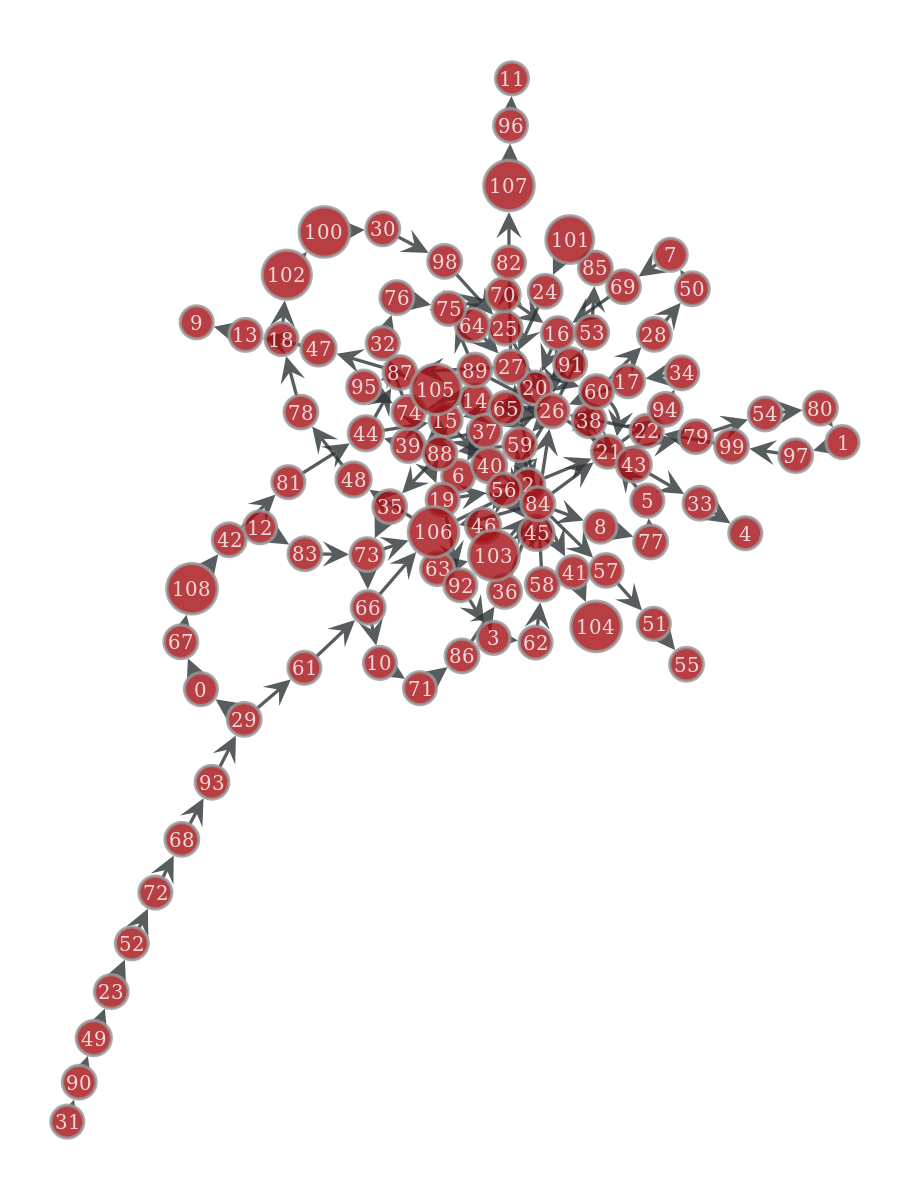
\includegraphics[scale=0.3]{germanwordgraphnumbered.png}
	\caption{}
	\label{fig:gernum}
\end{subfigure}
\caption{The German  (a) word graph and (b) numbered equivalent of the word graph generated from the German translation of the "Sleeping Beauty" corpus.}
\label{fig:gergraph}
\end{figure}

\begin{table}[H]
\centering
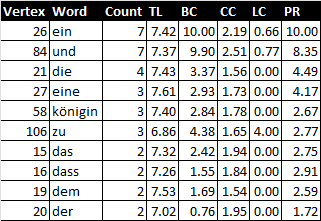
\includegraphics[scale=1]{germantabletop10.png}
\caption{Top 10 words with the highest frequency in the German translation of the corpus. Shown in table format with other graphical properties. }
\label{table:germantop}
\end{table}

Table \ref{table:germantop} shows the most common ten words in the German dataset along with each graph property value. The translation to English for each word in the order of the table is ``and", ``a" (Masculine), ``the" (Feminine), ``to", ``a" (Feminine), ``Queen", ``King", ``not", ``himself/herself/itself" (dependent on the pronoun this refers to) and ``the" (Neutral). As expected when comparing to the English dataset most words appear in both translations as the top ten, in particular the top three. Which we recall was ``and", ``the" and ``a" for the English dataset. However rather than a cumulative count of ``the" in English, the German translation has multiple versions. This may counteract each others importance and bring they values lower. By retaining the inflectable changes in grammar, the average count is lower for the German translation. Additionally the range of frequencies has also decreased from 9-1 to 7-1. For example, "the" in English was split into "die", "der" and "das" in German. By noting these key differences, the graphical properties will be analysed.

\begin{table}[H]
\centering
\begin{subtable}{.45\textwidth}
	\centering
	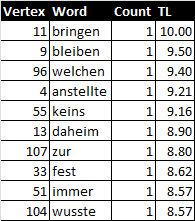
\includegraphics[scale=1]{gertabletctop.png}
	\caption{Top 10 works with highest trophic levels in the German translation dataset.}
	\label{table:germantoptc}
\end{subtable}
\hfill
\begin{subtable}{.45\textwidth}
	\centering
	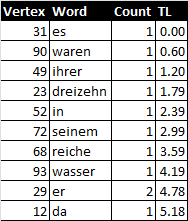
\includegraphics[scale=1]{gertabletcbot.png}
	\caption{Bottom 10 words ranked by their trophic levels based on the German Story Corpus.}
	\label{table:germanbottc}
\end{subtable}
\caption{Partial extracts of the table data for graphical properties of the German Story Corpus.}
\end{table}

Analysis of the trophic levels demonstrates that most words congregate at around 7.3. This can be more evidently seen in the graphical representations on Figures \ref{fig:gercentrality} and \ref{fig:gerother} later on. From the same graphs, there is a unique path from vertex 31 to 29 which is equivalent to the translation ``Es waren ihrer dreizehn in seinem Reiche, weil er". This path is grammatically correct and represents the beginning of a sentence belonging to the German story corpus. Furthermore this portion holds only unique words, hence has not been influenced by other vertices so demonstrates a clear hierarchical structure. Which is the reason the words used are of low trophic levels. Whereas most other sentences share words which causes the conglomeration nearer 7.3. Consequently the German language has more options for word choices which means the increased probability of unique sentences.

Trophic coherence has also benefited from the uniqueness of word choices since for the German graph, trophic coherence is calculated to be $0.29$. This is larger than the English graph which was $0.09$. Therefore the German graph has a clearer hierarchical structure compared to the English graph with clearer levels as demonstrated in further graphs below when analysing other properties.

\begin{table}[H]
\centering
\begin{subtable}{.2\textwidth}
	\centering
	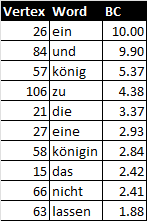
\includegraphics[scale=0.9]{germantablebc.png}
	\caption{}
	\label{table:germantablebc}
\end{subtable}
\hfill
\begin{subtable}{.2\textwidth}
	\centering
	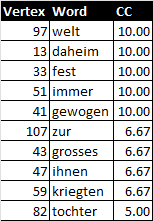
\includegraphics[scale=0.9]{germantablecc.png}
	\caption{}
	\label{table:germantablecc}
\end{subtable}
\hfill
\begin{subtable}{.2\textwidth}
	\centering
	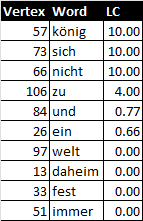
\includegraphics[scale=0.9]{germantablelc.png}
	\caption{}
	\label{table:germantablelc}
\end{subtable}
\hfill
\begin{subtable}{.2\textwidth}
	\centering
	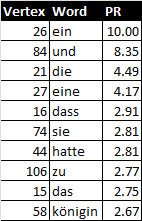
\includegraphics[scale=0.9]{germantablepr.png}
	\caption{}
	\label{table:germantablepr}
\end{subtable}
\caption{}
\label{table:germandata}
\end{table}

Entirety of the data presented in table form can be seen in Appendix \ref{app:}. Table \ref{table:germandata} (a)-(d) shows an extract of the top 10 complex values in order of highest to lowest for each property.

\begin{figure}[H]
\centering
\begin{subfigure}{.45\textwidth}
	\hspace{-1cm} 
	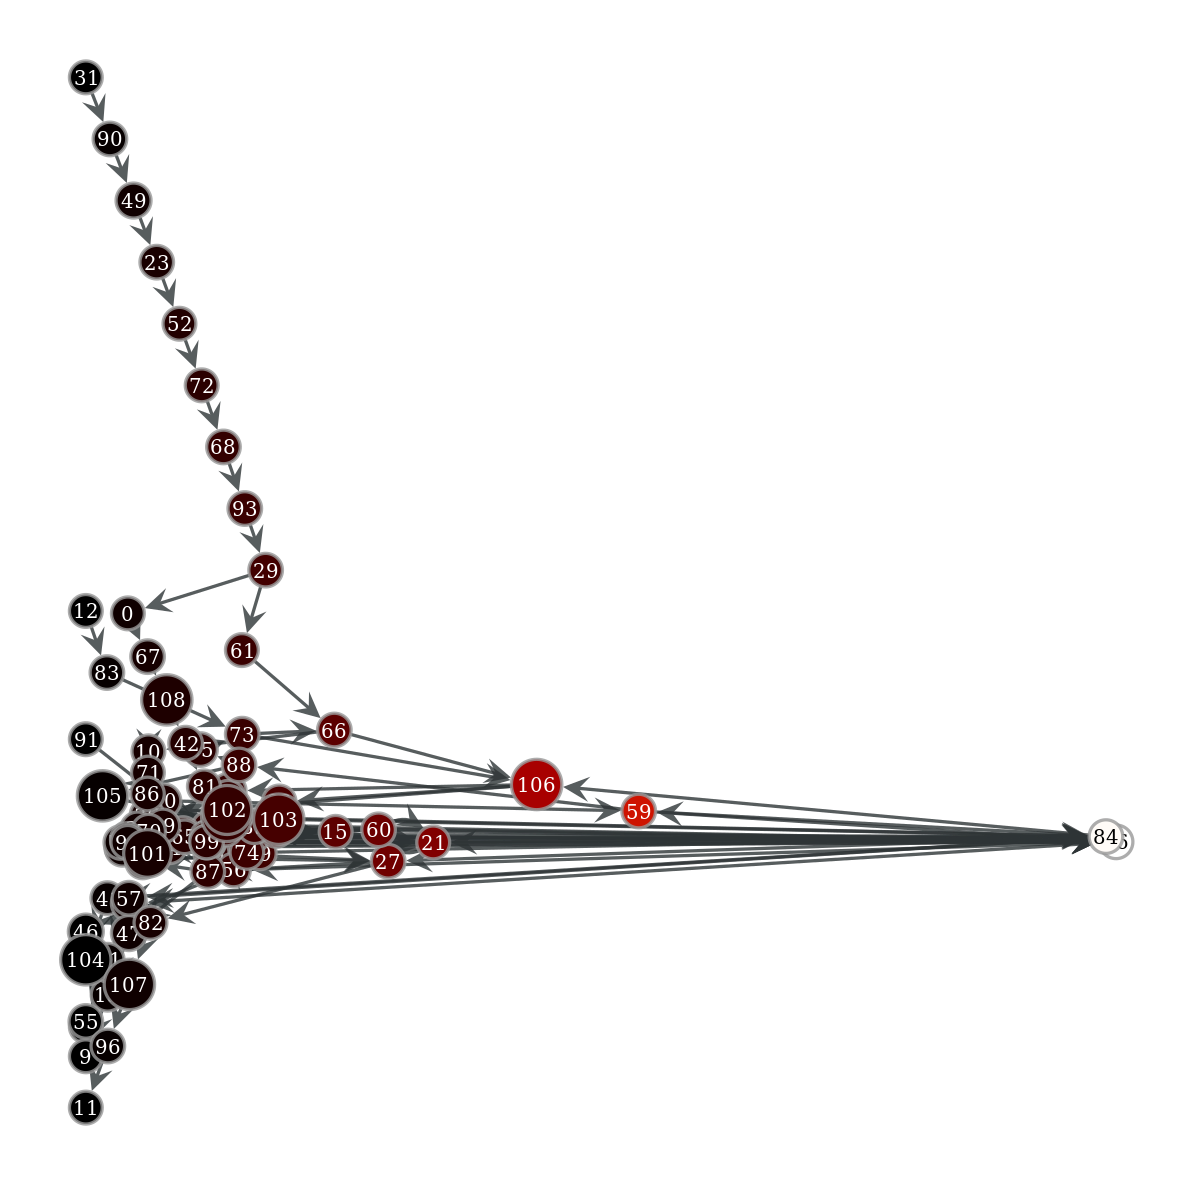
\includegraphics[scale=0.2]{germanbetweenness.png}
	\caption{Positions of the German numbered graph but with trophic levels and betweenness on the y-axis and x-axis respectively.}
	\label{fig:gerbc}
\end{subfigure}
\hfill
\begin{subfigure}{.45\textwidth}
	\hspace{-1cm} 
	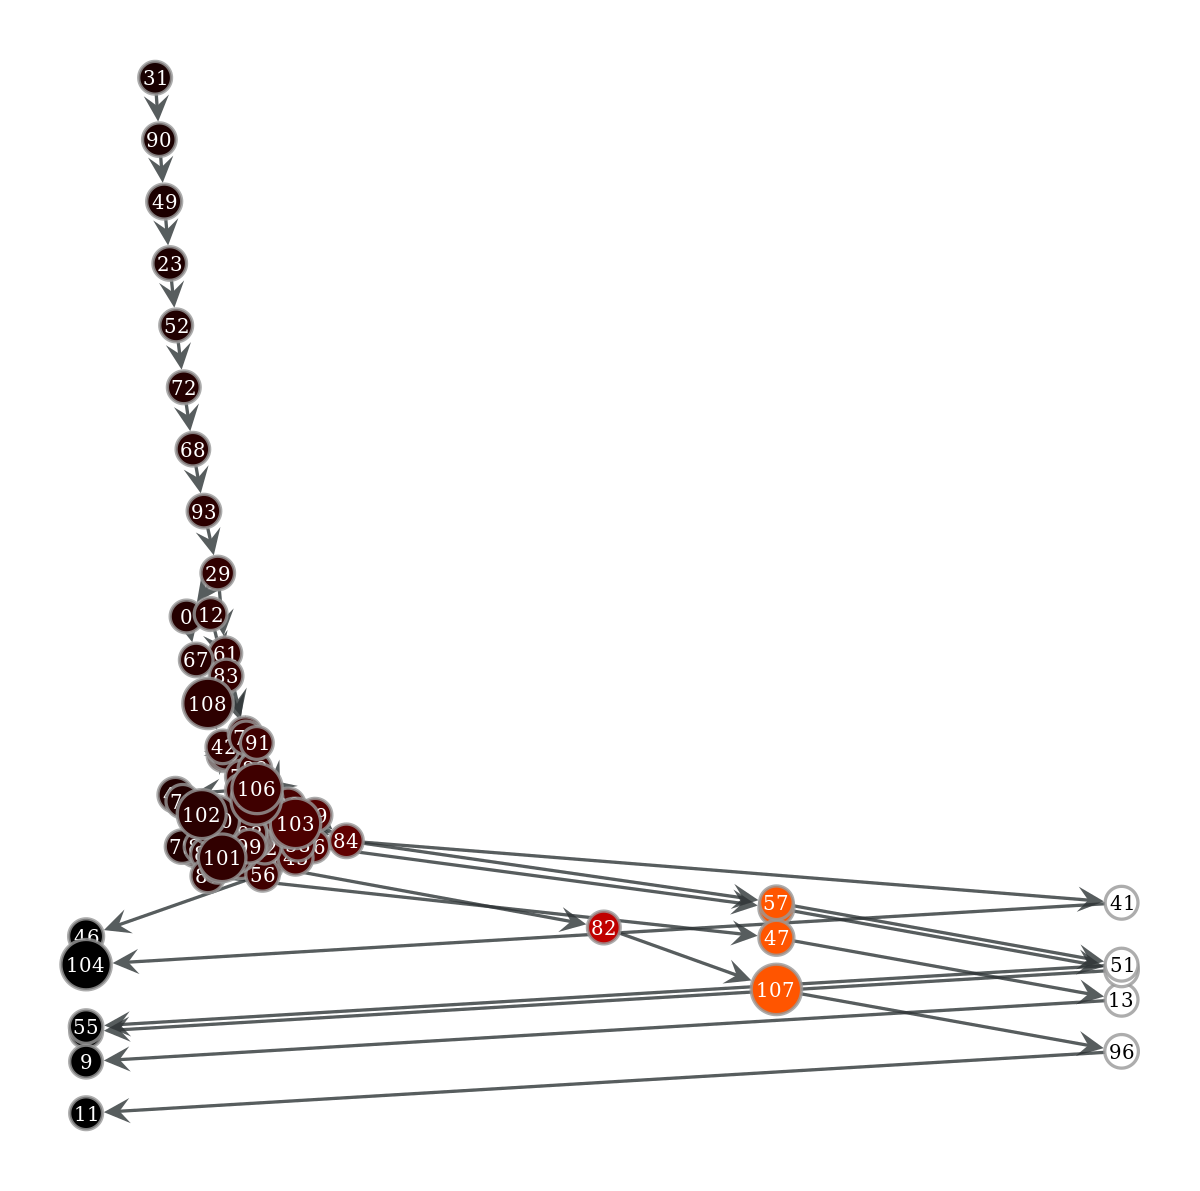
\includegraphics[scale=0.2]{germancloseness.png}
	\caption{Similar to the betweenness German graph but with closeness centrality values instead. }
	\label{fig:gercc}
\end{subfigure}
\caption{Betweenness and closeness centrality values displayed on the x-axis based on the German numbered word graph.}
\label{fig:gercentrality}
\end{figure}

Assessing the visual graphs (Figures \ref{fig:gerbc} and \ref{fig:gercc}), we identify vertex 84 and 26 who have the highest betweenness  values. A correlation to the frequencies of the words in the German Story Corpus can be seen through these vertices. Additionally, the same correlation was also true in the English version because the vertices in both versions referred to the words that are most commonly used as bridges or links in sentences. In the German case, the words are ``ein" and ``und".

With closeness centrality, it is a measure of influence on nearby words, the graph in Figure \ref{fig:gercc} shows that the vertices 97, 13, 33, 51 and 41 have the largest closeness values. These all correspond to the second to last word of each sentence apart from the first sentence which has the word ``Kind" as the second to last word. However ``Kind" is also used elsewhere meaning that its closeness value was influenced through other connections. The vertices of high closeness are unique and essential as a bridge in it's nearby words. Otherwise the neighbours of these vertices are likely to be isolated. Note that the orange vertices in Figure \ref{fig:gercc} are the unique words predecessors to the vertices of high closeness and the last word of every sentence always has a value of zero.

Therefore betweenness identifies the words of key importance that are used most commonly as connectors. Meanwhile closeness identifies the words most likely to isolate vertices of the graph when following the sentence flow, i.e. breaks up the rest of the sentence into unique words. Observe that the same pattern was seen in the English version but was set aside due to there being only one vertex of high closeness. However the German version shows a correlation of local importance to unique words which means that the English version may contain the same correlation.

\begin{figure}[H]
\centering
\begin{subfigure}{.45\textwidth}
	\hspace{-1cm} 
	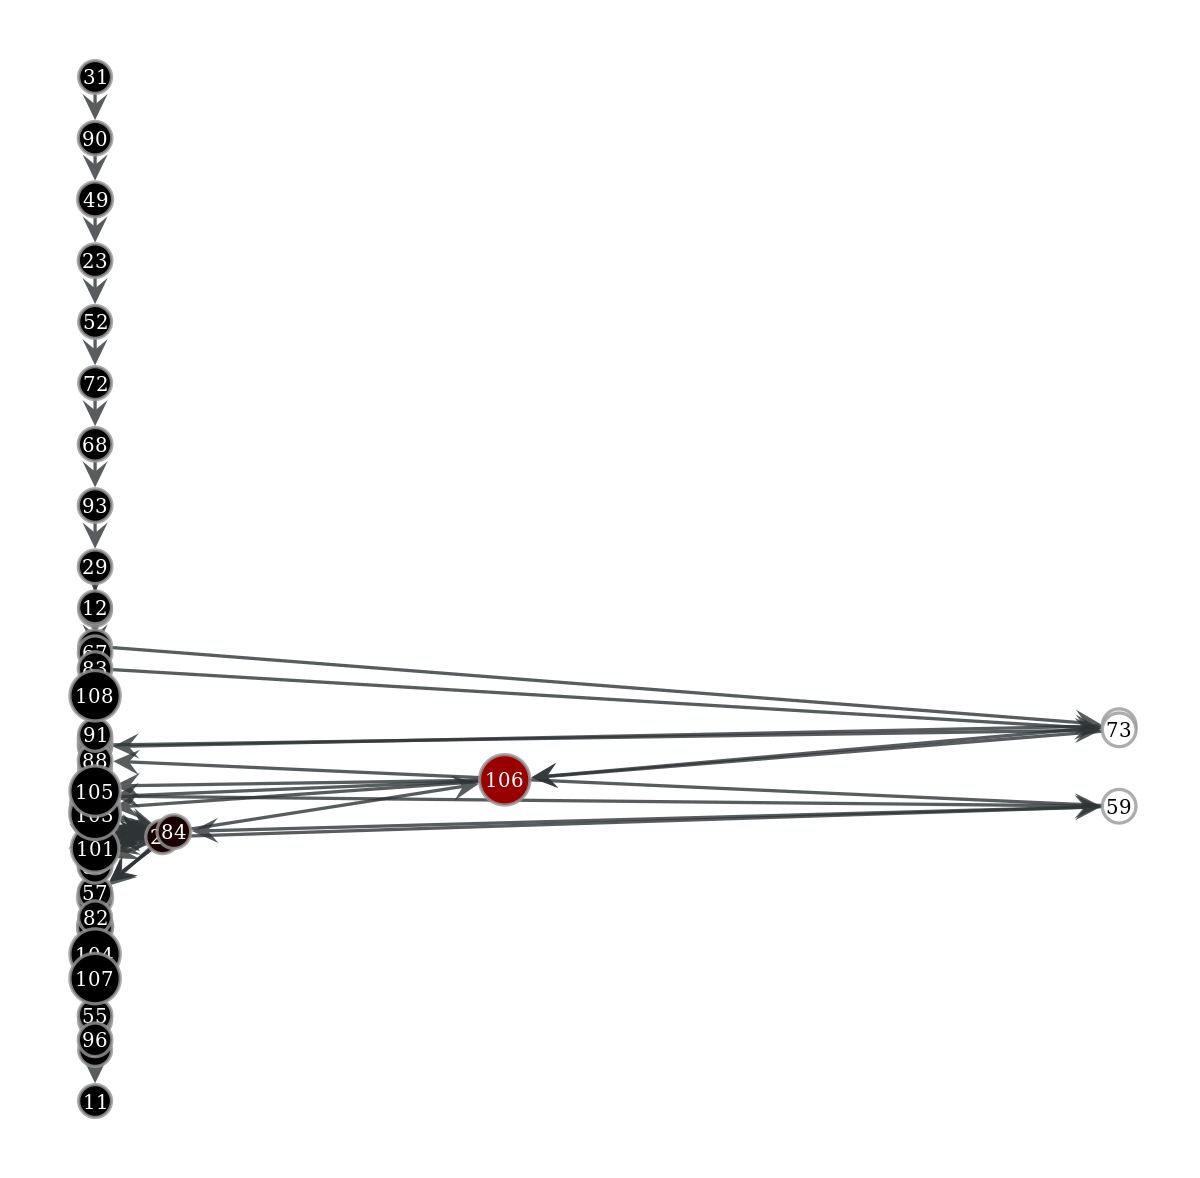
\includegraphics[scale=0.2]{germanlocalclustering.png}
	\caption{Displays the local clustering coefficient against the trophic levels.}
	\label{fig:gerlc}
\end{subfigure}
\hfill
\begin{subfigure}{.45\textwidth}
	\hspace{-1cm} 
	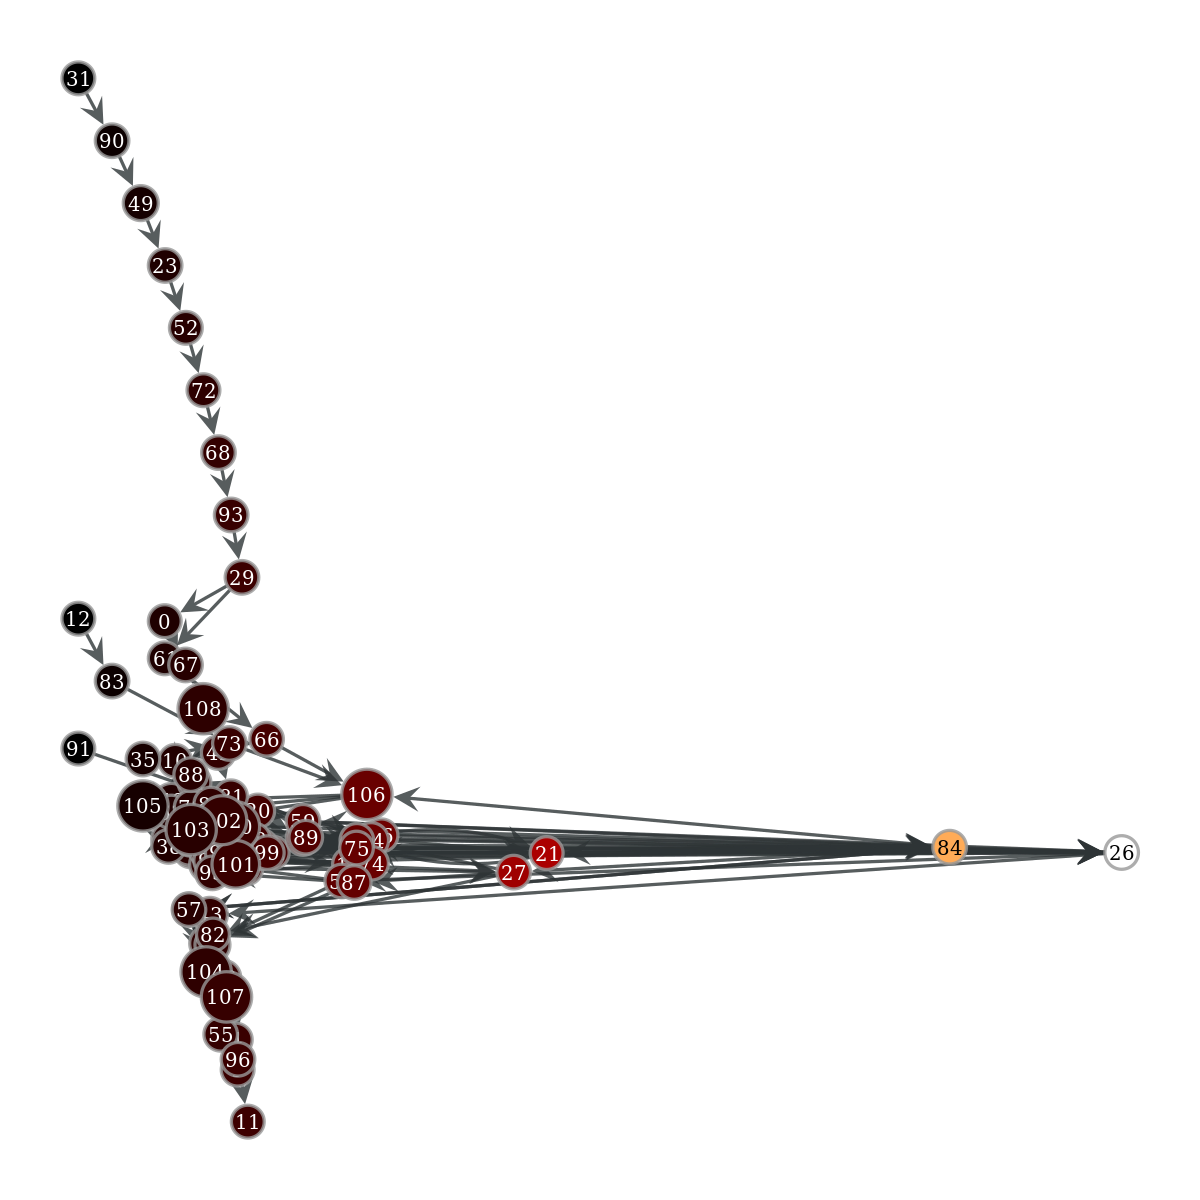
\includegraphics[scale=0.2]{germanpagerank.png}
	\caption{Displays the page rank against the trophic levels.}
	\label{fig:gerpr}
\end{subfigure}
\caption{Displays the local clustering and page rank on the x-axis instead of the centrality values.}
\label{fig:gerother}
\end{figure}

Nothing prominent can be derived by studying the local clustering coefficients (see Figure \ref{fig:gerlc}) because almost all vertices hold a local clustering coefficient of 0 apart from six vertices. Three of which are the vertices 57, 73 and 66 which corresponds to the words ``könig", ``sich" and ``nicht" respectively. These are not unique words in the German story corpus and no other vertices demonstrate anything unique with its local coefficient. 
On the other hand, vertices with a high page rank (see Figure \ref{fig:gerpr}) correlate to either conjunctions, vertex 84 (``und"), or words that accompany other words like pronouns or articles, vertices 26 (``ein"), 27 (``eine") etc. Therefore high page rank relates to key words that are used frequently in German, which remains true when extended to the German language as a whole.

In conclusion, similar results were seen when analysing the graphical properties based on the German and English translations. With German having a clearer visualisation and stronger correlation compared to the English language due the the uniqueness of inflectional words.

\subsection{French}
English and German are Germanic languages under the Indo-European family. Instead of another Germanic language, we study a different branch under the Indo-European family. The language being French which lies under the Italic branch of the same family. Similarly to German, French contains the same parts of speech as English but also inflectional words. So words can be inflected by number (singular or plural), gender, person, case, aspect and mood. However whilst German has three genders (Masculine, Feminine and Neutral), French \cite{hawkins2015french} only uses two, masculine and feminine. 

The story corpus is translated into the French version so graphs can be generated off this. Where the initial word graphs are shown in Figure \ref{fig:fregraph}. 

\begin{figure}[H]
\centering
\begin{subfigure}{.45\textwidth}
	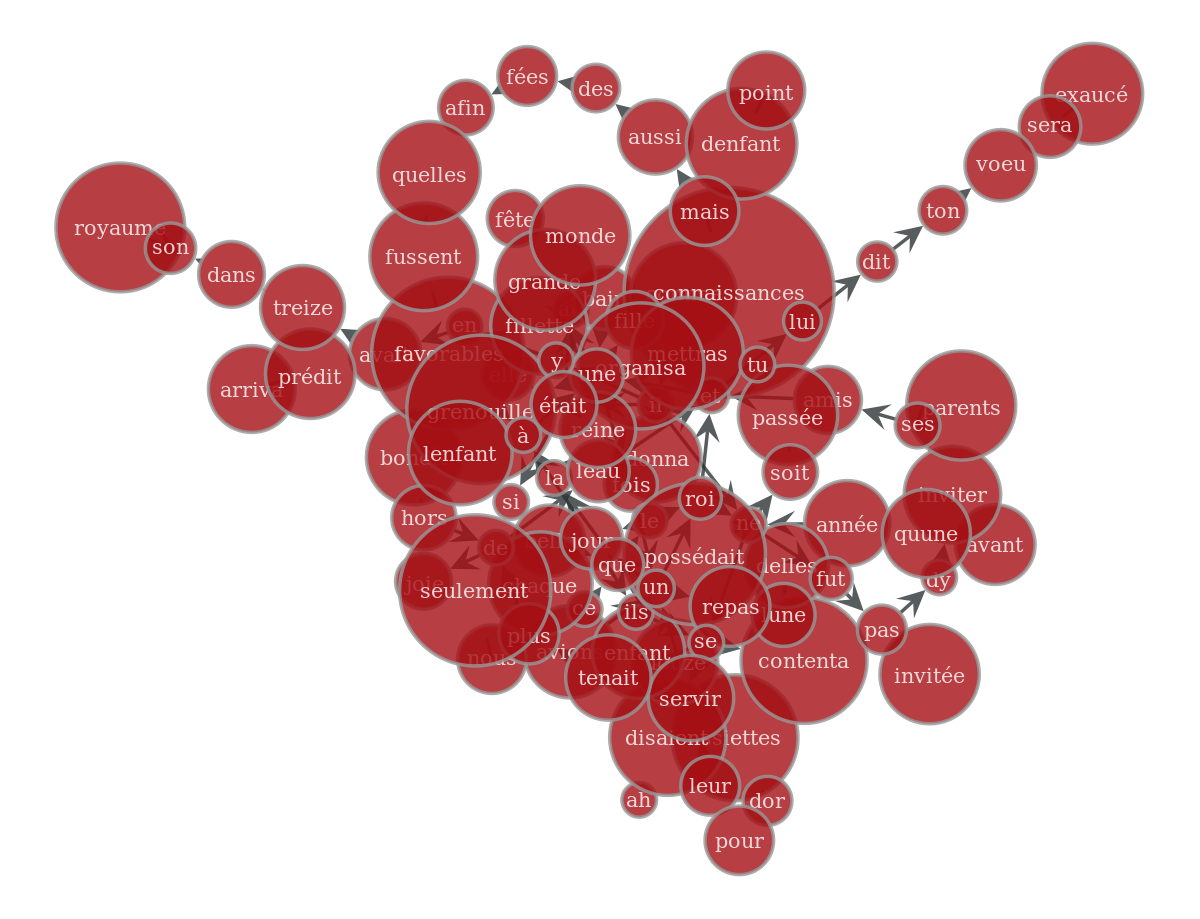
\includegraphics[scale=0.2]{frenchwordgraph.png}
	\caption{French word graph generated based on the French translation of the corpus.}
	\label{fig:freword}
\end{subfigure}
\hfill
\begin{subfigure}{.45\textwidth}
	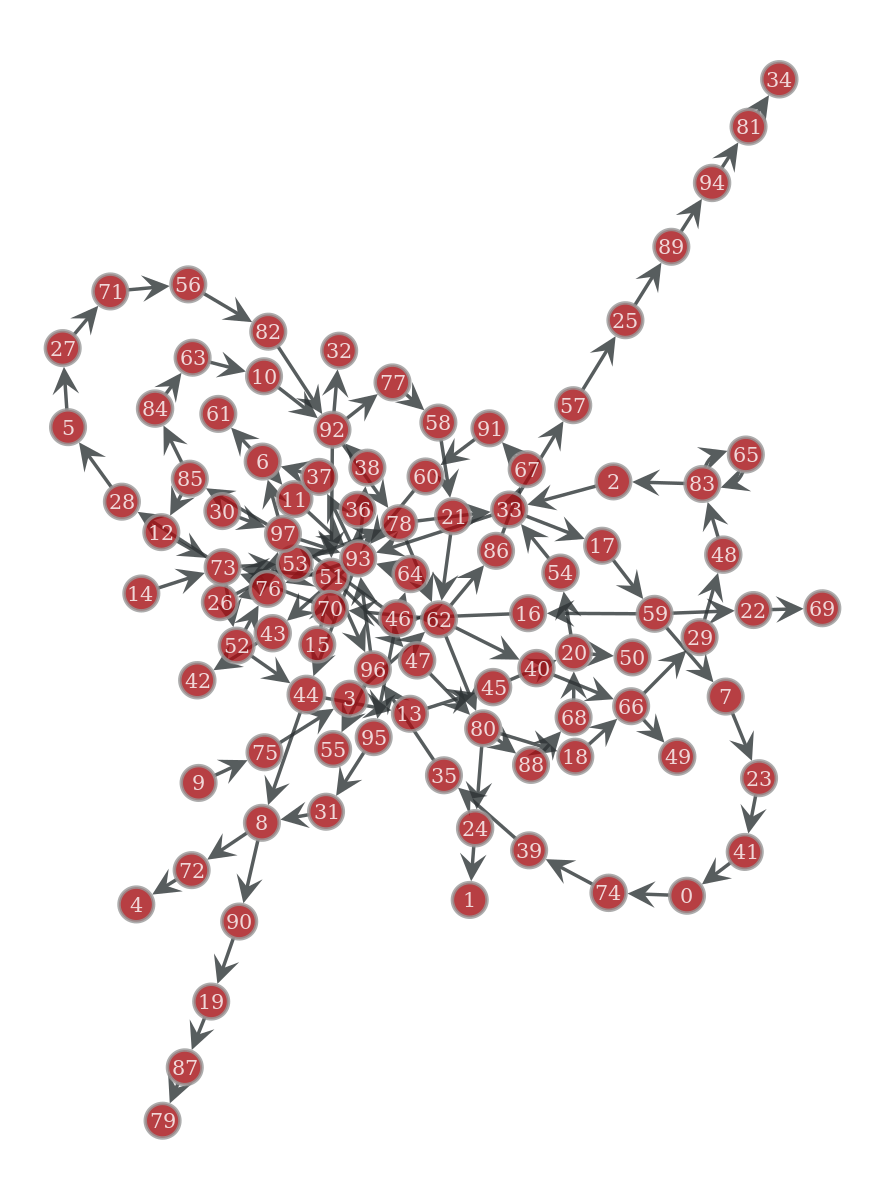
\includegraphics[scale=0.2]{frenchwordgraphnumbered.png}
	\caption{Numbered version of the word graph to provide a clearer graph. This is called the French numbered graph.}
	\label{fig:frenum}
\end{subfigure}
\caption{The French word graph and numbered equivalent of the word graph generated from the French translation of the "Sleeping Beauty" corpus.}
\label{fig:fregraph}
\end{figure}

\begin{table}[H]
\centering
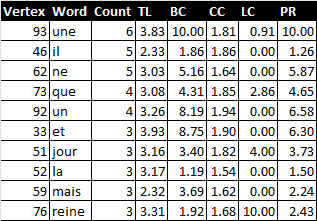
\includegraphics[scale=1]{frenchtabletop10.png}
\caption{Top 10 words with the highest frequency in the French translation of the corpus. Shown in table format with other graphical properties. }
\label{table:frenchtop}
\end{table}

Words of highest frequency are shown in the extract Table \ref{table:frenchtop} where the majority of words seen are inflectable and used as a way to give more information. Such as the particle of vertex 93 meaning a/an or vertex 46 meaning he/it. So these would be used more frequently and it is generally true for the French language.

\begin{table}[H]
\centering
\begin{subtable}{.45\textwidth}
	\centering
	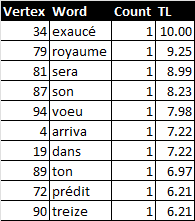
\includegraphics[scale=1]{frenchtabletctop.png}
	\caption{Top 10 works with highest trophic levels in the French translation dataset.}
	\label{table:frenchtoptc}
\end{subtable}
\hfill
\begin{subtable}{.45\textwidth}
	\centering
	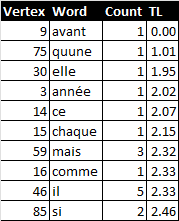
\includegraphics[scale=1]{frenchtabletcbot.png}
	\caption{Bottom 10 words ranked by their trophic levels based on the French Story Corpus.}
	\label{table:frenchbottc}
\end{subtable}
\caption{Partial extracts of the table data for graphical properties of the French Story Corpus.}
\end{table}

In relation to the story corpus, French has a high trophic coherence which is calculated to be $0.36$ which is higher than both English and German. Even though it may not be close to 1, in comparison to previous languages, a clearer level structure can be identified for the French language. Top 10 trophic levels can be seen in Table \ref{table:frenchtoptc} where the high values represent the words nearer to the end of a sentence. All top 10 are within the last four words of sentences in the story corpus. However the predecessors of the words have an impact on their trophic level. If the predecessors of a word is involved in other sentences at a earlier stage then the predecessors trophic value will be lowered. Subsequently lowering the trophic levels of the neighbourhood of the word. This can be seen by vertex 49 who has a trophic level of 5.08 even though it is last in its sentence.

\begin{table}[H]
\centering
\begin{subtable}{.27\textwidth}
	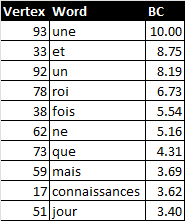
\includegraphics[scale=0.9]{frenchtablebc.png}
	\caption{}
	\label{table:frenchtablebc}
\end{subtable}
\hfill
\begin{subtable}{.2\textwidth}
	\centering
	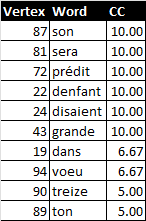
\includegraphics[scale=0.9]{frenchtablecc.png}
	\caption{}
	\label{table:frenchtablecc}
\end{subtable}
\hfill
\begin{subtable}{.2\textwidth}
	\centering
	\includegraphics[scale=0.9]{frenchtablelc.png}
	\caption{}
	\label{table:frenchtablelc}
\end{subtable}
\hfill
\begin{subtable}{.2\textwidth}
	\centering
	\includegraphics[scale=0.9]{frenchtablepr.png}
	\caption{}
	\label{table:frenchtablepr}
\end{subtable}
\caption{}
\label{table:frenchdata}
\end{table}

Tables \ref{table:frenchdata} (a)-(d) shows an top 10 extract of Table \ref{app:} in the order of their corresponding graph property value.

\begin{figure}[H]
\centering
\begin{subfigure}{.45\textwidth}
	\hspace{-1cm} 
	\includegraphics[scale=0.2]{frenchbetweenness.png}
	\caption{Positions of the French numbered graph but with trophic levels and betweenness on the y-axis and x-axis respectively.}
	\label{fig:frbc}
\end{subfigure}
\hfill
\begin{subfigure}{.45\textwidth}
	\hspace{-1cm} 
	\includegraphics[scale=0.2]{frenchcloseness.png}
	\caption{Similar to the betweenness French graph but with closeness centrality values instead. }
	\label{fig:frcc}
\end{subfigure}
\caption{Betweenness and closeness centrality values displayed on the x-axis based on the French numbered word graph.}
\label{fig:frcentrality}
\end{figure}

Vertices with high betweenness will have many other vertices that must connect to it in order to reach other vertices within their sentence. As mentioned in previous language analysis, betweenness helps identify the key bridges in the sentences by finding the vertices which control the majority of the flow of data. Furthermore the betweenness coincides with the frequency. On the other hand there are vertices such as vertex 78 ("roi") and vertex 38 ("fois") who have a betweenness value of 6.73 and 5.54 (see Table \ref{table:frenchtablebc})respectively but only a count of 2 and 1. By further analysis, the reason they have high betweenness, is that they are used with a predecessor and successor of higher betweenness value, i.e. "un roi et" and "une fois un". Consequently causing its own betweenness value to be inflated because "un", "et" and "une" must pass through "roi" or "fois" to complete their word pathing. Therefore, if vertices have a low count but are connected to other vertices of high betweenness, then their values will relatively increased.

As discovered in the German analysis, closeness centrality identifies the vertices most likely divide the graph from their directed path, i.e. the words most likely to isolate the remaining sentence. Otherwise vertices are involved in a diverse range of sentences causing a high degree where the formation of vertex conglomerates can be seen (see Figure \ref{fig:frcc} where a clustering of vertices is shown in the upper left quadrant). Studying the graph in Figure \ref{fig:frcc}, French words have more vertices with a variety of high closeness values. The graph shows clearly that vertices of high closeness would cause isolation for further vertices along it's path. According to the visualisations, French is the most unique language out of the three languages seen so far as there is a higher number of clear divisions in the closeness values.

\begin{figure}[H]
\centering
\begin{subfigure}{.45\textwidth}
	\hspace{-1cm} 
	\includegraphics[scale=0.2]{frenchlocalclustering.png}
	\caption{Displays the local clustering coefficient against the trophic levels.}
	\label{fig:frlc}
\end{subfigure}
\hfill
\begin{subfigure}{.45\textwidth}
	\hspace{-1cm} 
	\includegraphics[scale=0.2]{frenchpagerank.png}
	\caption{Displays the page rank against the trophic levels.}
	\label{fig:frpr}
\end{subfigure}
\caption{Displays the local clustering and page rank on the x-axis instead of the centrality values.}
\label{fig:frother}
\end{figure}

Finally the local clustering coefficients and page rank. Only two vertices have a local clustering coefficient of 10 which are vertex 53 ``le" and vertex 76 ``reine" (see Figure \ref{fig:frlc} and Table \ref{table:frenchtablelc}). In the context of French, nothing particular can be derived. However when studying the graphs of local clustering in various languages, the vertices with a local clustering value are never an start or end to a branch.

Page ranks for the French story corpus measures the influence the vertices have on one another other than for their immediate neighbours. This is why vertex 46 "il" has a low page rank value of 1.26 as it is located at the start of the sentence so does not have enough unique vertices encompassing it to be influential.

In conclusion, French has similar results in comparison to English and German which makes sense as they are a part of the same language family. So to see a different perspective, the study of other language families are undertaken such as the Japonic language family.

\section{Japonic}
The Japonic language family is the protolanguage for Japanese and Ryūkyūan languages \cite{vovin2017origins} so it is a relatively small language family compared to other language families. Translating the corpus into Japanese gives us a new dataset to use for graph property analysis which will be studied in comparison to the previous language family.
\subsection{Japanese}
To give a larger variety of languages, Japanese is studied as it uses vastly different grammar compared to the languages seen so far. Japanese has only five lexical word classes which includes nouns, verbal nouns, nominal adjectives, verbs and adjectives. The order in which the words are structured is different to Indo-European languages since Japanese uses SOV (Subject-Object-Verb) compared to languages like German and English which uses SVO (Subject-Verb-Object). Furthermore Japanese does not rely heavily on grammatical number or gender and is more focused on their system of honorifics which indicates the speaker, listener or person of reference. Therefore, even if Japanese contains words borrowed from other languages (these are referred to as \emph{loanwords} \cite{miura1979influence}), their grammar is vastly different. 

We follow the same process as before and input the Japanese Story corpus into my program to produce the basic graphs. For simplicity, we show the numbered version of the word graph (see Figure \ref{fig:jpgraph}) with the words they correspond to in the full table of data (See Table \ref{app:}).

\begin{figure}[H]
\centering
\includegraphics[scale=0.25]{japanesewordgraph.png}
\caption{The Japanese word graph and numbered equivalent of the word graph generated from the Japanese translation of the "Sleeping Beauty" corpus.}
\label{fig:jpgraph}
\end{figure}

\begin{table}[H]
\centering
\includegraphics[scale=1]{japanesetabletop10.png}
\caption{Top 10 words with the highest frequency in the Japanese translation of the corpus. Shown in table format with other graphical properties. }
\label{table:japanesetop}
\end{table}

Out of the previous languages, the larger frequency of a words appearance was 9. With Japanese, there are 6 words with 11 or more appearances (see Table \ref{table:japanesetop}), largest being vertex 17 with 14 appearances. Vertex 17 represents a form of conjugation which means that their use depends on the inflections of it's associated words. Generally vertex 17 is most commonly used to signify the past tense. So rather than having a separate word for different tenses, Japanese uses specific accompanying words which leads to their frequency being significantly higher. Additional examples such as vertex 12 who has a large frequency and its associated word is used to empathically add more information (an empathic and). Vertex 6 is a particle that means ``but" or indicates the sentence subject. Therefore, Japanese words have a heavy reliability on each other to define their overall meaning which is demonstrated by the many edges signifying these relationships.

\begin{table}[H]
\centering
\begin{subtable}{.45\textwidth}
	\centering
	\includegraphics[scale=1]{jptabletctop.png}
	\caption{Top 10 works with highest trophic levels in the Japanese translation dataset.}
	\label{table:japanesentoptc}
\end{subtable}
\hfill
\begin{subtable}{.45\textwidth}
	\centering
	\includegraphics[scale=1]{jptabletcbot.png}
	\caption{Bottom 10 words ranked by their trophic levels based on the Japanese Story Corpus.}
	\label{table:japanesebottc}
\end{subtable}
\caption{Partial extracts of the table data for graphical properties of the Japanese Story Corpus.}
\end{table}

Due to the graph having an increased amount of bidirectional edges such as the edge between vertex 25 and 5. As well as an increased amount of self loops, the trophic incoherence is very high in comparison to previous languages. Thus, the trophic coherence for the Japanese extract is only $0.04$. Caused by the ambiguity of hierarchical structure with bidirectional edges and self loops. An example of a self loop is vertex 0 which is part of the word ``everyday". The subsequent repetition of a word that creates a different meaning is known as \emph{reduplication}.

Unfortunately without a full understanding of the Japanese language, direct analysis of each word is difficult. This is because of the multitude of meanings each word has depending on the context. Therefore, the trophic levels can only provide a generic flow of text from lowest trophic levels (see Table \ref{table:japanesebottc}) as sentence starters to highest levels (see Table \ref{table:japanesetoptc})  as sentence enders.

\begin{table}[H]
\centering
\begin{subtable}{.2\textwidth}
	\centering
	\includegraphics[scale=0.9]{japanesetablebc.png}
	\caption{}
	\label{table:japanesetablebc}
\end{subtable}
\hfill
\begin{subtable}{.2\textwidth}
	\centering
	\includegraphics[scale=0.9]{japanesetablecc.png}
	\caption{}
	\label{table:japanesetablecc}
\end{subtable}
\hfill
\begin{subtable}{.2\textwidth}
	\centering
	\includegraphics[scale=0.9]{japanesetablelc.png}
	\caption{}
	\label{table:japanesetablelc}
\end{subtable}
\hfill
\begin{subtable}{.2\textwidth}
	\centering
	\includegraphics[scale=0.9]{japanesetablepr.png}
	\caption{}
	\label{table:japanesetablepr}
\end{subtable}
\caption{}
\label{table:japanesedatar}
\end{table}

As with previous languages, Tables \ref{table:japanesedatar} (a)-(d) are ordered extracts from the main table in Appendix \ref{app:}.

\begin{figure}[H]
\centering
\begin{subfigure}{.45\textwidth}
	\hspace{-1cm} 
	\includegraphics[scale=0.2]{japanesebetweenness.png}
	\caption{Positions of the Japanese numbered graph but with trophic levels and betweenness on the y-axis and x-axis respectively.}
	\label{fig:jpbc}
\end{subfigure}
\hfill
\begin{subfigure}{.45\textwidth}
	\hspace{-1cm} 
	\includegraphics[scale=0.2]{japanesecloseness.png}
	\caption{Similar to the betweenness Japanese graph but with closeness centrality values instead. }
	\label{fig:jpcc}
\end{subfigure}
\caption{Betweenness and closeness centrality values displayed on the x-axis based on the Japanese numbered word graph.}
\label{fig:jpcentrality}
\end{figure}

The graphs in the centrality Figure \ref{fig:jpcentrality} shows that the words are more evenly distributed unlike the Indo-European languages. Which correlates to the importance of the Japanese characters nature of being reliant on one another for their meaning and demonstrates the complexities of the language visually. The basic correlations from other languages still hold here. Although further detail cannot be determined by the visualisation other than importance.

Japanese's closeness centrality values also has a larger average compared to the Indo-European languages. Instead of looking at the vertices in relation to the whole graph, closeness focusses on the closer clusters. Hence provides a similar shape betweenness but shifted right to emphasise the zooming in on the vertices. There are no vertices that stand out so no correlations can be easily derived.

Therefore only a general correlation can be demonstrated through the centrality graphs. Clearer results can be gathered with Japanese fluency.

\begin{figure}[H]
\centering
\begin{subfigure}{.45\textwidth}
	\hspace{-1cm} 
	\includegraphics[scale=0.2]{japaneselocalclustering.png}
	\caption{Displays the local clustering coefficient against the trophic levels.}
	\label{fig:jplc}
\end{subfigure}
\hfill
\begin{subfigure}{.45\textwidth}
	\hspace{-1cm} 
	\includegraphics[scale=0.2]{japanesepagerank.png}
	\caption{Displays the page rank against the trophic levels.}
	\label{fig:jppr}
\end{subfigure}
\caption{Displays the local clustering and page rank on the x-axis instead of the centrality values.}
\label{fig:jpother}
\end{figure}

Local clustering coefficients (see Figure \ref{fig:jplc}) measures how close the vertex is part of a unique directed triangle, i.e. a directed 3 cycle. The vertices 29, 87 and 61 are vertices who are involved in such triangles where they each have a unique in and out edge to other vertices. Lower values means they are less likely to be involved in unique triangles. Thus local clustering can identify certain triples in the Japanese texts that would have unique meanings. 

Page rank identifies the vertices who have an influence to other vertices nearby but not immediate neighbours like what closeness does. However nothing further can be correlated based on this graph (see Figure \ref{fig:jppr}).

In conclusion the way the Japanese story corpus is split into the database (character by character), only general correlations can be determined based upon the graphs and their properties. Stronger links as to what exact words have importance cannot be obtained here without the full understanding of the language. On the other hand, we see that in general the graphs are different to the ones based on the Indo-European languages which demonstrates the languages differences. To see this further we analyse another language and it's language family.

\section{Sino-Tibetan}
Sino-Tibetan is the final language family in which we analyse and contains over 400 languages. Two groups of languages that are successors of this family are the Tibeto-Burman language group and Chinese language group. Focus on the Chinese language will be taken to translate the story corpus into. Mandarin Chinese is chosen here since it is the 2nd most spoken language after English.

\subsection{Chinese}
The main branches of Chinese are Mandarin or Cantonese with Mandarin considered to be the standard and is the official language of China. Mandarin is also the language in which the corpus was translated into but will refer to this as Chinese for simplicity. Chinese has a SVO (subject-verb-object) sentence structure like with English. However the language is made up of syllables \cite{ross2017modern} rather than words. Syllables come with 3 parts, an initial consonant, the tone, and a final. These parts determines the meaning to each syllable and instead of writing their unique characters, they can be written using Pinyin. Pinyin is the standard system for romanised spelling and a useful tool in learning Chinese and their pronunciations. A simple word like ``hello" is ``nǐ hǎo" in Pinyin where ``n" and ``h" are initials, ``i" and ``ao" are finals and the accents on the letters ``i" and ``a" are the tone for the syllables. The tone matches the pitch of the syllable and leads to different meanings for the each word. Although each syllable in Chinese has its own definitions, they can be combined to form a different word. E.g. In Pinyin, ``dì" means earth but "dì tú" means map.

Similarly to Japanese, Chinese has very few inflectional characters and utilises other particles to accompany the syllables so various verbal aspects can be expressed. Another similarity is the use of reduplication where a syllable is repeated to give a different meaning. Parts of speech for Chinese is split into two major categories, the \emph{function} words and the \emph{content} words. The function words contains nouns, pronouns, verbs, auxiliary verbs, adjectives, number words, measure words, interjections and onomatopoeias. Function words contain conjunctions, prepositions and particles. Furthermore, each subgroup mentioned can have further branches dependent on the context that they are used in. For example, nouns can be proper nouns, location nouns, place nouns and time nouns in the Chinese language.

Therefore Chinese contains a larger amount of unique syllables compared to the words in the English language. Also syllables have a reliability factor and depends on the context of use (like when studying Japanese). Keeping this in mind, we generate and analyse the graphs beginning with seeing the basic word graph generated for the Chinese translation of the story corpus, seen in Figure \ref{cngraph} (shown with integer labelling to reference each word of the entire table, Table ?? in the Appendix).

\begin{figure}[H]
\centering
\includegraphics[scale=0.3]{chinesewordgraph.png}
\caption{The Chinese word graph and numbered equivalent of the word graph generated from the Chinese translation of the "Sleeping Beauty" corpus.}
\label{fig:cngraph}
\end{figure}

\begin{table}[H]
\centering
\includegraphics[scale=1]{chinesetabletop10.png}
\caption{Top 10 words with the highest frequency in the Chinese translation of the corpus. Shown in table format with other graphical properties. }
\label{table:chinesetop}
\end{table}

The syllables with the highest count (see Table \ref{table:chinesetop}) is vertex 90 which is ``de" in Pinyin. This is a particle so has a grammatical meaning with different functions to denote possession. Also can be accompanied by other parts of speech. Other syllables with high counts include vertex 71, ``yǒu", vertex 5, ``gè" and vertex 0, ``yī". These vertices all have various meanings depending on their use, ``yǒu" can mean ``have", ``is" and ``are", ``gè" can mean ``this", ``that", the party of a specific size or a classifier for people or objects. Vertex 0, ``yī", can mean ``a" or is a part of a number like ``1" in the English language. Therefore the syllables with a high count represents the words of varied meanings which are important in the sentence structure or identifiers for words with different genders.

\begin{table}[H]
\centering
\begin{subtable}{.45\textwidth}
	\centering
	\includegraphics[scale=1]{cntabletctop.png}
	\caption{Top 10 works with highest trophic levels in the Chinese translation dataset.}
	\label{table:chinesetoptc}
\end{subtable}
\hfill
\begin{subtable}{.45\textwidth}
	\centering
	\includegraphics[scale=1]{cntabletcbot.png}
	\caption{Bottom 10 words ranked by their trophic levels based on the Chinese Story Corpus.}
	\label{table:chinesebottc}
\end{subtable}
\caption{Partial extracts of the table data for graphical properties of the Chinese Story Corpus.}
\end{table}

An increased amount of reduplications and bidirectional edges appear in the Chinese graph. Like before with the Japanese data, trophic levels do not demonstrate a clear visual hierarchy. Meaning that the trophic coherence is low and is calculated to be $0.09$ based on the Chinese translation of the story corpus. Therefore average positions of each syllable within a sentence can still be represented but with minor flexibility. The trophic levels go from low to high in relation to the sentence flow with Table \ref{table:chinesetoptc} showing the top 10 syllables nearer the start of a sentence and Table \ref{table:chinesebottc} showing the top 10 syllables for the end. Grammatically correct can be seen by unique downward paths in the graph visualisations such as the path from vertex 19 to vertex 61 (see Figure \ref{fig:cncentrality} or \ref{fig:cnother}).

\begin{table}[H]
\centering
\begin{subtable}{.2\textwidth}
	\centering
	\includegraphics[scale=0.9]{chinesetablebc.png}
	\caption{}
	\label{table:chinesetablebc}
\end{subtable}
\hfill
\begin{subtable}{.2\textwidth}
	\centering
	\includegraphics[scale=0.9]{chinesetablecc.png}
	\caption{}
	\label{table:chinesetablecc}
\end{subtable}
\hfill
\begin{subtable}{.2\textwidth}
	\centering
	\includegraphics[scale=0.9]{chinesetablelc.png}
	\caption{}
	\label{table:chinesetablelc}
\end{subtable}
\hfill
\begin{subtable}{.2\textwidth}
	\centering
	\includegraphics[scale=0.9]{chinesetablepr.png}
	\caption{}
	\label{table:chinesetablepr}
\end{subtable}
\caption{}
\end{table}

The top 10 syllables for each complex graph property is seen here where the full table is in Appendix \ref{app:}.

\begin{figure}[H]
\centering
\begin{subfigure}{.45\textwidth}
	\hspace{-1cm} 
	\includegraphics[scale=0.2]{chinesebetweenness.png}
	\caption{Positions of the Chinese numbered graph but with trophic levels and betweenness on the y-axis and x-axis respectively.}
	\label{fig:cnbc}
\end{subfigure}
\hfill
\begin{subfigure}{.45\textwidth}
	\hspace{-1cm} 
	\includegraphics[scale=0.2]{chinesecloseness.png}
	\caption{Similar to the betweenness Chinese graph but with closeness centrality values instead. }
	\label{fig:cncc}
\end{subfigure}
\caption{Betweenness and closeness centrality values displayed on the x-axis based on the Chinese numbered word graph.}
\label{fig:cncentrality}
\end{figure}

Betweenness centrality in the Chinese translation Story corpus (see figure \ref{fig:cnbc}) identified the syllables vertex 90 and vertex 10 (both are particles) to be of high importance. Re-emphasizing the fact that they are the syllables that act most like bridges and needed to derive further meaning. Hence betweenness relate closely to the counts of the syllables discussed earlier. The same correlation is achieved in previously discussed languages so we can conclude that this correlation of importance holds for the majority of languages.

As mentioned in the German analysis, closeness measures the importance of words directly around them. In other words, the vertices vital in the paths structure (controlling the flow of data). Therefore, demonstrated by Figure \ref{fig:cncentrality}, vertex 98 has the highest closeness as without this vertex, vertex 61 is isolated. Subsequently the predecessors of vertex 98 have higher closeness. However there are no other vertices with high closeness since other syllables hold connections to various unique vertices. Thus inferring that these syllables of high degree have multiple meanings rather than the unique meaning of vertex 98s section of the path.

\begin{figure}[H]
\centering
\begin{subfigure}{.45\textwidth}
	\hspace{-1cm} 
	\includegraphics[scale=0.2]{chineselocalclustering.png}
	\caption{Displays the local clustering coefficient against the trophic levels.}
	\label{fig:cnlc}
\end{subfigure}
\hfill
\begin{subfigure}{.45\textwidth}
	\hspace{-1cm} 
	\includegraphics[scale=0.2]{chinesepagerank.png}
	\caption{Displays the page rank against the trophic levels.}
	\label{fig:cnpr}
\end{subfigure}
\caption{Displays the local clustering and page rank on the x-axis instead of the centrality values.}
\label{fig:cnother}
\end{figure}

By taking what we found in the Japanese graphs, we now know that the local clustering coefficient identifies vertices involved in unique directed 3-cycles. For example, vertex 22 is uniquely part of the directed 3-cycle, vertex 0 $\rightarrow$ 22 $\rightarrow$ 71 $\rightarrow$ 0 where vertex 22 is seen as the pinnacle of the cycle because vertices 22 and 71 hold other edge connections within the graph seen in Figure \ref{fig:cnlc}. The same applies to vertex 94 as it is involved in its own directed 3-cycle. So local clustering does not identify the vertices of high importance but rather certain triples within the corpus.

The page rank (see Figure \ref{fig:cnpr}) identifies the vertices with influence to vertices other than their immediate neighbours. Evidently vertices with high betweenness will also have a high page rank as they are more commonly used in the corpus. Similar results have been seen with other languages for page ranks so evidently, page rank and betweenness values are close in the context of lexical analysis.



\chapter{Conclusion}
Based upon the five of the nine total languages shown in the previous chapter. Results achieved in the previous chapter demonstrated the similarities of languages within the same family, particularly French and German. Their uniqueness could also be seen when comparing the graphs of each language as they each varied. Especially with languages of a different family as the Indo-European were all clustered together more but the Japonic and Sino-Tibetan families were much more evenly distributed. 

Therefore the study of complex graphical properties such as trophic coherence, various centrality values and clustering have proved beneficially in distinguishing graphs from one another as well as a tool to represent possible information based upon the graph.  

We summarise each graph property and the correlations that were derived from them in the next section.

\section{Final Correlations}
Based on each graph property that was studied, we take their correlations within the story corpus used and summarised as follows.

\subsection{Local Clustering Coefficient}
Local clustering with the lexical graphs corresponded to words that would most likely be involved in triples (a 3-cycle). However because of the common reuse of words, there were usually no triples that represented anything unique to the language. A way to improve the usefulness of local clustering in lexical analysis would be to use use specific motifs that could prove to generate a better correlation. Currently a generic 3-cycle is used for the local clustering calculations so using specific motifs may generate interesting results..

\subsection{Betweenness Centrality}
Betweenness centrality was chosen as it identifies the vertices with most control of informational flow. In the context of language analysis, betweenness values corresponded to the most commonly used words in each language which is further proven by the Zipf curve as mentioned in the English analysis. This was further verified when compared with the frequency of the words/vertices for every language dataset.

\subsection{Closeness Centrality}
Closeness centrality determines the vertices that on average have the shortest connections to all the other vertices within the graph. For lexical analysis, closeness centrality correlated to the vertices whom are most likely to isolate the rest of its sentence. This may be because the rest of the sentence uses more unique words which means that the vertex of high closeness is the closest to these words as well as the previous words whom did not have a high closeness. Therefore the reason these such vertices had a high closeness and its correlation in lexical terms.

\subsection{Page Rank}
Page ranks finds the vertices who are seen as important by finding the backlinks that refer to the vertex and other vertices which reference these vertices. This is similar to betweenness as both identified the vertices that held the most importance within the text so the ranks were similar to the betweenness but has more reference to the predecessors of the vertices. This causes the slight different of the betweenness graph and the page rank graph.

\subsection{Trophic Level}
Finally tropic levels are useful in determining structure and flow in a graph. Within lexical analysis, the flow of the sentences were represented by the ranges of trophic levels which were normalised to 0-10 like with the other values. Consequently were used as the y-positioning downwards from 0-10 so that the sentence flow was represented correctly. Trophic levels for each vertex represented the average position that they belonged to within a sentence with 0 at the start and 10 at the end. Languages with better sentence structure had more evenly distributed levels due to the fact that their sentence length was not as varied to other languages. 

Additionally, through trophic levels visualisation, each graph property in the previous chapter had key subsegments of the y-range which held the relative graph properties high value. For example, in the betweenness graphs, the vertices of high betweenness value were centralised which means that they appeared most commonly in the middle of sentences. This is grammatically true because words of importance either appeared as a bridge in a sentence like "and" or are used commonly throughout the sentence. Thus leading to an average closer to the centre. A similar trend was seen with local clustering where the vertices/words of high local clustering were lower in the y-range.
\\

\noindent In conclusion, each graph property have been researched for their use and benefits within a graph. The calculations for each complex graphical property was also given along with the possible variations which depended on the graph types. I.e. the weights, whether the graph is directed, self loops, etc. After detailed descriptions of various properties were given, specific ones were transferred and used on text corpora based on various different languages and their corresponding language family. This was possible through the use of programming in Python code to generate a dataset from a text input (the story corpus for each language). The dataset can then be used to formalise a graph so that the calculations for each complex graph property can be calculated from. Furthermore, the values of each property are normalised and applied onto the positions of each vertex to generate a new graph that provides a visual representation for the dataset. Each new graph represents a different complex graph property which achieves the aim of my research. Therefore the newly generated visualisations of the graph have proven to be useful in analysis and to highlight key components of interest by showing them as extremes of clusters within the new graph. Results found can then be expanded onto a larger dataset to predict the key areas of the larger text such as the words that would be of interest. This also means that when given another graph of the same language but with unknown vertices, the graph generated based on the corpus can be used to predict and identify what the unknown vertices could be. 

\section{Further works and Applications}
Briefly mentioned in the last part, the visualisations can be used as a prediction tool within the same language as similar vertices that represent each word would correspond to a similar location in this visualisation. As well as this expansion, the visualisation can be used to analyse new or unknown languages through the comparison of graphs since languages of the same family produce graphs that have resemblances. Once the best language family is chosen, predictions of what components of the graph represents can be given from the facts of other languages within the same language family. Improvements for each specific language representations can be remedied since languages such as Japanese and Chinese does not use words as their sentence structure is more complex than most other languages.

Therefore the current works on lexical analysis and complex graph properties can be taken further by introducing unknown languages, expanding on the graph properties mentioned such as using specific motifs for the local clustering or the application onto other subject areas rather than lexical analysis.

Other areas that could be analysed includes neuroscience. The brain \cite{de2014graph} can be regarded as a complex network of neurons where each vertex represents units or specific regions and the edges represents the links or connections between them. Analysis of neurological diseases such as schizophrenia, dementia and Alzheimer's can be used to generated relative graph visualisations. These visualisations can be studied further to find common links and correlations within each neurological disease so that action could be taken if early signs of similar correlations are found within a healthy brain. A similar idea was studied based on detecting changes in the brain which has Alzheimer's using graph theory \cite{10.1093/braincomms/fcaa129}.
In conclusion graph theory is crucial in representing various types of information in the real world from friendship groups to the complex structures of the brain. Many subject areas can be represented as a graph which means that they can undergo similar graphical analysis and visualisations which experimented on in Chapters 3 and 4 to deduce correlations and key components of interest in the relative graph.


\bibliography{references}
\bibliographystyle{unsrt}

\begin{appendices}
\chapter{Karate Club}
\section{Karate Club Adjacency Matrix}\label{app:karateadj}
This is the adjacnency matrix generated for the karate club dataset.
\begin{figure}[H]
	\centering
	\includegraphics[scale=0.55]{karatematrix.png}
\end{figure}

\chapter{Langauages}
\section{Text Corpus}
\begin{quote}
In times past there lived a king and queen, who said to each other every day of their lives, "Would that we had a child!" and yet they had none. But it happened once that when the queen was bathing, there came a frog out of the water, and he squatted on the ground, and said to her: "Thy wish shall be fulfilled; before a year has gone by, thou shalt bring a daughter into the world."

And as the frog foretold, so it happened; and the queen bore a daughter so beautiful that the king could not contain himself for joy, and he ordained a great feast. Not only did he bid to it his relations, friends, and acquaintances, but also the wise women, that they might be kind and favourable to the child. There were thirteen of them in his kingdom, but as he had only provided twelve golden plates for them to eat from, one of them had to be left out.
\end{quote}
\subsection{foo title}
Some text

\end{appendices}

\end{document}
